% !TeX program = pdflatex
\documentclass[11pt]{article}

% Encoding and fonts
\usepackage[utf8]{inputenc}
\usepackage[T1]{fontenc}
\usepackage{lmodern}

% Maths and symbols
\usepackage{amsmath,amssymb}

% Graphics & tables
\usepackage{graphicx}
\usepackage{float} % Required for [H] figure placement
\usepackage{placeins} % For \FloatBarrier command
% \usepackage{booktabs} % Removed for compatibility

% Hyperlinks
\usepackage[hidelinks]{hyperref}

% Page geometry
\usepackage{geometry}
\geometry{margin=1in}

% Unicode symbols support
\usepackage{textcomp}
\usepackage{xspace}

% Definition for ≤ symbol
\DeclareUnicodeCharacter{2264}{$\leq$}

%-----------------------------------------------------------------------------
% Title information author list
%-----------------------------------------------------------------------------
\title{Comparative Analysis of Single--Neuron versus Dual--Neuron Output Layers in Binary Classification Neural Networks}
\author{Khadim Hussain\\Department of Computer Science \\ University of Southern Punjab, Pakistan\\[1ex]\textit{(bsf2004901@ue.edu.pk)}}
\date{May 11, 2025}

%-----------------------------------------------------------------------------
\begin{document}
\maketitle

\begin{abstract}
Binary classification is a classic problem in machine learning: given an input, the model predicts one of two outcomes. In binary classification, neural networks have traditionally implemented a single-output neuron with sigmoid activation. However, an equally valid alternative is to assign two output neurons with a softmax activation function. This study extensively compares the two architectural options with respect to their effect on the performance of models, their training dynamics, and generalization capabilities. From extensive experimentation on benchmark datasets across diverse neural network architectures, we probe under what conditions each approach might find favor. These observations add to knowledge with respect to design considerations for neural networks performing binary classification tasks.
\end{abstract}

\section{Introduction}
It is very common in the context of neural networks to handle binary classification problems through a single output neuron employing sigmoid activation; outputs nearing 0 are denoting a particular class while outputs approaching 1 are considered of the opposite type. Such a convention can definitely be abandoned; the second way to go about it consists of employing two output neurons under softmax activation, clearly modeling both the positive and "background" classes. Theoretically, both the configurations can solve the same problems, but it is the performance characteristics, training dynamics, and generalization capabilities using the different approaches that could possibly be different.

In this research, we try to systematically explain the difference between the two approaches and their influence on other qualities of model performance. We investigate whether the greater expressiveness afforded by the two-neuron output layer is truly an advantage or whether the single-neuron approach, with less expressiveness, presents some benefits of regularization and generalization.

\section{Background and Related Work}

\subsection{Neural Network Output Layers for Classification}
Binary classification in neural networks has been historically implemented using one single output neuron with a  sigmoid activation [4]. The sigmoid function maps  output value of the networkbetween 0 and 1, which can be considered as the probability of the positive class. This approach is mathematically accurate and directly tied to logistic regression.

The alternative another approach uses two output neurons with softmax activation, which produces a probability distribution over the two classes [6]. While this is the standard approach for multi-class classification problems, its application to binary problems is less common in neural network architectures but theoretically possible.

Variants of these two-neuron softmax design have also been explored for binary problems. Memisevic et al. [6] introduced gated softmax in their work while Tyagi et al. [5] revisited the sigmoid–versus-softmax debate and showed that a properly tuned sigmoid–MSE objective can outperform softmax–cross-entropy. Further more investigations include Yang et al. [13], Klimo et al. [14], Maharjan et al. [15], and Hu et al. [16], which explore alternative loss functions, error-detecting output codes, and hardware-efficient softmax implementations.

\subsection{Related Research}
Prior research on binary image classification can be grouped into three types: \textbf{output-layer configurations}, \textbf{Vision Transformer (ViT) models}, and \textbf{optimisation \& activation-function studies}.

\textbf{Output-layer configurations.} The classical choice is a single sigmoid neuron, which directly models the Bernoulli probability of the positive class [4]. Variants of the two-neuron softmax design have also been explored for binary problems. Memisevic et al. [6] introduced gated softmax, while Tyagi et al. [5] revisited the sigmoid-versus-softmax debate and showed that a properly tuned sigmoid–MSE objective can outperform softmax–cross-entropy.

\textbf{Vision Transformers.} Dosovitskiy et al.'s seminal ViT work [1] demonstrated that pure transformer architectures can match or surpass CNNs on large-scale image classification. Comprehensive surveys [2, 3] and data-efficient variants such as DeiT [11] together with the study by Khalil et al. [12] confirm ViT's competitiveness, motivating its inclusion in our comparison. The transformer paradigm itself originated with Vaswani et al. [20]. Additional surveys and architectural improvements—Khan et al. [17], the hierarchical Swin Transformer [18], Twins spatial-attention design [19], token-based Visual Transformers [21], comparative reviews [22], privacy-preserving ViT applications [24], and ViT image-classification case studies [23] further demonstrate the breadth of transformer-based methods for image classification.

\textbf{Optimisation and activation functions.} Learning dynamics are also created by the non linearity used in the hidden layers. Large empirical benchmarks [7, 8] and theoretical analyses [9, 10] highlight the strengths and weaknesses of ReLU, Swish, Softplus and related functions. Interrelated studies of Softplus units [25], activation-function comparisons on MNIST [26], empirical analyses across vision tasks [27], and broader surveys [28] provide additional context on activation choice.

\subsection{Summary of Related Literature}

Table~\ref{tab:literature_summary1} and Table~\ref{tab:literature_summary2} present a comprehensive overview of key papers relevant to our research on binary classification output layer configurations and neural network architectures.

\begin{table}[htbp]
\scriptsize
\centering
\caption{Summary of related work on vision transformers and neural architectures}
\label{tab:literature_summary1}
\begin{tabular}{|c|p{1.8cm}|p{2.5cm}|p{2.5cm}|p{2.2cm}|p{2.5cm}|}
\hline
\textbf{\ S.No} & \textbf{Author(s) \& Year} & \textbf{Title} & \textbf{Method/Model} & \textbf{Dataset} & \textbf{Key Findings} \\ 
\hline
1 & Dosovitskiy et al., 2020 & An Image is Worth 16×16 Words: Transformers for Image Recognition at Scale & Vision Transformer (ViT) & ImageNet, CIFAR-100, VTAB & 88.55\% accuracy on ImageNet with ViT-H/14 \\ 
\hline
2 & Wang et al., 2025 & Vision Transformers for Image Classification: A Comparative Survey & Comparative survey & ImageNet, CIFAR-10/100, JFT-300M & ViT-B/16: 77.9\%, DeiT-S: 79.8\% \\ 
\hline
3 & Han et al., 2023 & A Survey on Vision Transformer & Survey of Vision Transformers & Various vision tasks & ViTs perform competitively with CNNs \\ 
\hline
4 & Yang et al., 2018 & Binary Output Layer of Feedforward Neural Networks for Multi-Class Classification & Binary output layer approach & MNIST, multi-class datasets & Better accuracy with fewer nodes \\ 
\hline
5 & Tyagi et al., 2024 & Making Sigmoid-MSE Great Again: Output Reset Challenges Softmax Cross-Entropy & MSE with sigmoid and Output Reset & MNIST, CIFAR-10, Fashion-MNIST & MSE matches or outperforms cross-entropy \\ 
\hline
6 & Memisevic et al., 2010 & Gated Softmax Classification & Gated Softmax (log-bilinear model) & MNIST variations, rectangles & Competitive error rates \\ 
\hline
7 & Eger et al., 2019 & Is it Time to Swish? Comparing Deep Learning Activation Functions & Comparison of 21 activation functions & NLP tasks (MR, SUBJ, TREC) & Penalized tanh most stable across tasks \\ 
\hline
8 & Jagtap \& Karniadakis, 2022 & How important are activation functions in regression and classification? & Survey of activation functions & MNIST, CIFAR-10/100, PIML datasets & ReLU variants excel in classification \\ 
\hline
9 & Asadi \& Jiang, 2020 & On Approximation Capabilities of ReLU Activation and Softmax Output Layer & Theoretical analysis & N/A (theoretical work) & Universal approximation theorems \\ 
\hline
10 & Dubey et al., 2021 & Activation Functions in Deep Learning: A Comprehensive Survey & Survey of 18 activation functions & CIFAR10/100, IWSLT, WMT & Task-specific optimal activation functions \\ 
\hline
11 & Touvron et al., 2021 & Training data-efficient image transformers \& distillation through attention & Data-efficient image Transformers (DeiT) & ImageNet, CIFAR-10/100 & DeiT-B: 83.1\% top-1 accuracy \\ 
\hline
12 & Khalil et al., 2023 & A Comprehensive Study of Vision Transformers in Classification Tasks & Various Vision Transformers & ImageNet, CIFAR-10/100 & ViT-H/14: 88.55\% on ImageNet \\ 
\hline
13 & Yang et al., 2020 & Binary Output Layer of Extreme Learning Machine & ELM with binary approach & Various classification tasks & Binary approach uses fewer output nodes \\ 
\hline
14 & Klimo et al., 2021 & Deep Neural Networks Classification via Binary Error-Detecting Output Codes & Zadeh fuzzy logic with CRC & CIFAR-10, MNIST, Fashion-MNIST & CRC7 achieved 92.44--93.97\% \\ 
\hline

\end{tabular}
\end{table}

\begin{table}[htbp]
\scriptsize
\centering
\label{tab:literature_summary2}
\begin{tabular}{|c|p{1.8cm}|p{2.5cm}|p{2.5cm}|p{2.2cm}|p{2.5cm}|}
\hline
15 & Maharjan et al., 2020 & A Novel Enhanced Softmax Loss Function for Brain Tumour Detection & CNN with modified softmax loss & Brain tumor images (3064 total) & Improved accuracy by ~2\% with faster processing \\ 
\hline
16 & Hu et al., 2018 & Efficient Hardware Architecture of Softmax Layer & Hardware optimization of softmax & Not specified & Hardware optimization of softmax \\ 
\hline
17 & Khan et al., 2022 & Transformers in Vision: A Survey & Survey of vision transformers & Various vision datasets & Comprehensive survey of ViTs \\ 
\hline
18 & Liu et al., 2021 & Swin Transformer: Hierarchical Vision Transformer & Swin Transformer & ImageNet-1K, COCO, ADE20K & 87.3\% top-1 accuracy on ImageNet-1K \\ 
\hline
19 & Chu et al., 2021 & Twins: Revisiting Spatial Attention in Vision Transformers & Twins-PCPVT and Twins-SVT architectures & Various vision tasks & Strong performance across vision tasks \\ 
\hline
20 & Vaswani et al., 2017 & Attention Is All You Need & Transformer architecture & Translation datasets & 27.5 BLEU on English-German translation \\ 
\hline
21 & Wu et al., 2020 & Visual Transformers: Token-based Image Representation & Visual Transformer (VT), VT-ResNets & ImageNet, COCO-stuff, LIP & 4.6--7 points improvement over ResNet \\ 
\hline
22 & Maurício et al., 2023 & Comparing Vision Transformers and CNNs & Literature review & Various benchmarks & ViT better with noisy data; CNN better with small datasets \\ 
\hline
23 & Huo et al., 2023 & Vision Transformer Applications in Classification & Various ViT applications & Not accessible & Applications to image classification \\ 
\hline
24 & Qi et al., 2022 & Privacy-Preserving Image Classification Using Vision Transformer & ViT with block-wise encryption & CIFAR-10, CIFAR-100 & 96.64\% accuracy on CIFAR-10 \\ 
\hline
25 & Zheng et al., 2015 & Improving Deep Neural Networks Using Softplus Units & Softplus activation & Various datasets & Benefits of softplus activation \\ 
\hline
26 & Pedamonti, 2018 & Comparison of Non-Linear Activation Functions & DNNs with various activations & MNIST & ELU achieved up to 98.3\% on MNIST \\ 
\hline
27 & Alcantara, 2017 & Empirical Analysis of Non-Linear Activation Functions & DNNs with various activations & MNIST & ELU with learning rate 0.02 achieved 98.0\% \\ 
\hline
28 & Sharma et al., 2017 & Activation Functions in Neural Networks & Survey of activation functions & Various applications & Survey of common activation functions \\ 
\hline
\end{tabular}
\end{table}


\textbf{Our contribution.}  In contrast to previous studies, we provide the first systematic comparison of single- versus dual-neuron outputs across three architectures (Small CNN, ViT, ResNet-50) under identical hyper-parameters. Our results show a statistically significant advantage ($p = 0.0027$) of the single-neuron design in accuracy, F1, and AUC while incurring no additional computational cost.

\section{Methodology}
\subsection{Research Questions}
This study addresses the following key questions:
\begin{enumerate}
\item Does the choice between single-neuron and dual-neuron output configurations affect model accuracy, precision, recall, and F1 score in binary classification tasks?
\item Are there any differences in convergence speed, stability, or learning dynamics between single-neuron and dual-neuron models?
\item Does one approach (single-neuron or dual-neuron) generalize better to unseen data than the other?
\item Are there any specific types of binary classification problems or neural architectures where one approach consistently outperforms the other?
\end{enumerate}

\subsection{Experimental Setup}
We conduct experiments using several popular neural network architectures:
\begin{itemize}
\item A custom small CNN
\item Vision Transformer (ViT)
\item ResNet50
\end{itemize}

Each architecture is implemented with both output configurations:
\begin{itemize}
\item Single neuron with sigmoid activation
\item Two neurons with softmax activation
\end{itemize}

For training and evaluation, we use binary classification tasks derived from the CIFAR-10 dataset, creating multiple binary classification problems by pairing different classes (e.g., airplane vs. automobile, cat vs. dog).

\subsection{Training and Evaluation Protocol}
All models are trained using the following protocol:
\begin{itemize}
\item Optimization: Adam optimizer
\item Loss functions: Binary cross-entropy for single-neuron models, categorical cross-entropy for two-neuron models
\item Learning rate scheduling: Reduce on plateau
\item Early stopping to prevent overfitting
\item Data augmentation: Standard image augmentation techniques
\end{itemize}

We evaluate models using:
\begin{itemize}
\item Accuracy, precision, recall, and F1 score
\item ROC curves and AUC
\item Training and validation loss curves
\item Confusion matrices
\end{itemize}

\subsection{Dataset and Split Details}
All experiments use the CIFAR-10 dataset (60 000 colour images, 32×32 px, 10 classes). Following the standard train/test split we retain the original 50 000 training images and 10 000 test images. For each binary task we:
\begin{itemize}
\item \textbf{Class filtering} Select only the two target classes (IDs listed in Table 2) from both the training and test partitions.
\item \textbf{Validation split} Apply an internal 90 / 10 split on the filtered training set (\texttt{train\_test\_split} with \texttt{random\_state = 42}) to obtain validation data. The resulting sample counts per task are therefore 9 000 (train) / 1 000 (val) / 2 000 (test).
\item \textbf{Mutual exclusivity} Because the validation set is carved out of the training data (after class filtering) and the CIFAR-10 test partition is disjoint by design, \textit{no image appears in more than one split}.
\end{itemize}

\textbf{Table 2: Binary classification tasks used in our experiments.}

\begin{tabular}{lll}
\hline
Task ID & Class Pair & CIFAR-10 Class IDs \\
\hline
1 & Airplane vs. Automobile & 0 vs. 1 \\
2 & Cat vs. Dog & 3 vs. 5 \\
3 & Frog vs. Ship & 6 vs. 8 \\
\hline
\end{tabular}

\textbf{Pre-processing steps}
\begin{itemize}
\item \textbf{Resize} All images are resized to the model‐specific input resolution (32×32 for Small CNN, 224×224 for ViT and ResNet-50).
\item \textbf{Normalisation} \texttt{mean=[0.485,0.456,0.406]}, \texttt{std=[0.229,0.224,0.225]} (ImageNet statistics).
\item \textbf{Augmentation (train only)} Random horizontal flip, rotation (±15°), colour jitter, and random affine translation (≤10 \%).
\end{itemize}

\subsection{Hyper-parameter Configuration}
\textbf{Table 1: Hyper-parameter configuration used in all experiments.}

\begin{tabular}{ll}
\hline
Hyperparameter & Value \\
\hline
Optimiser & Adam \\
Initial learning rate & 0.001 \\
Weight decay & 1 × 10$^{-4}$ \\
LR scheduler & ReduceLROnPlateau (factor = 0.2, patience = 5, min\_lr = 1 × 10$^{-6}$) \\
Epochs & 15 (Small CNN = 20; default in code = 30 but early-stopping halted earlier) \\
Batch size & 32 (ViT cat vs dog = 16) \\
Early stopping patience & 10 \\
Image resolution & 32×32 (Small CNN) / 224×224 (ViT, ResNet-50) \\
Data augmentation & As listed in Sec. 3.4 \\
\hline
\end{tabular}

\subsection{Model Architectures}

To provide a comprehensive understanding of the neural network architectures used in our experiments, we present visual diagrams of each model design. These diagrams illustrate the layer configurations, connections, and key architectural features that distinguish each model.

\subsubsection{Small CNN Architecture}

Our custom Small CNN architecture represents a lightweight convolutional neural network designed specifically for this research. Figure~\ref{fig:small_cnn_arch} illustrates its structure with both single-neuron and dual-neuron output configurations.

\begin{figure}[htbp]
\centering
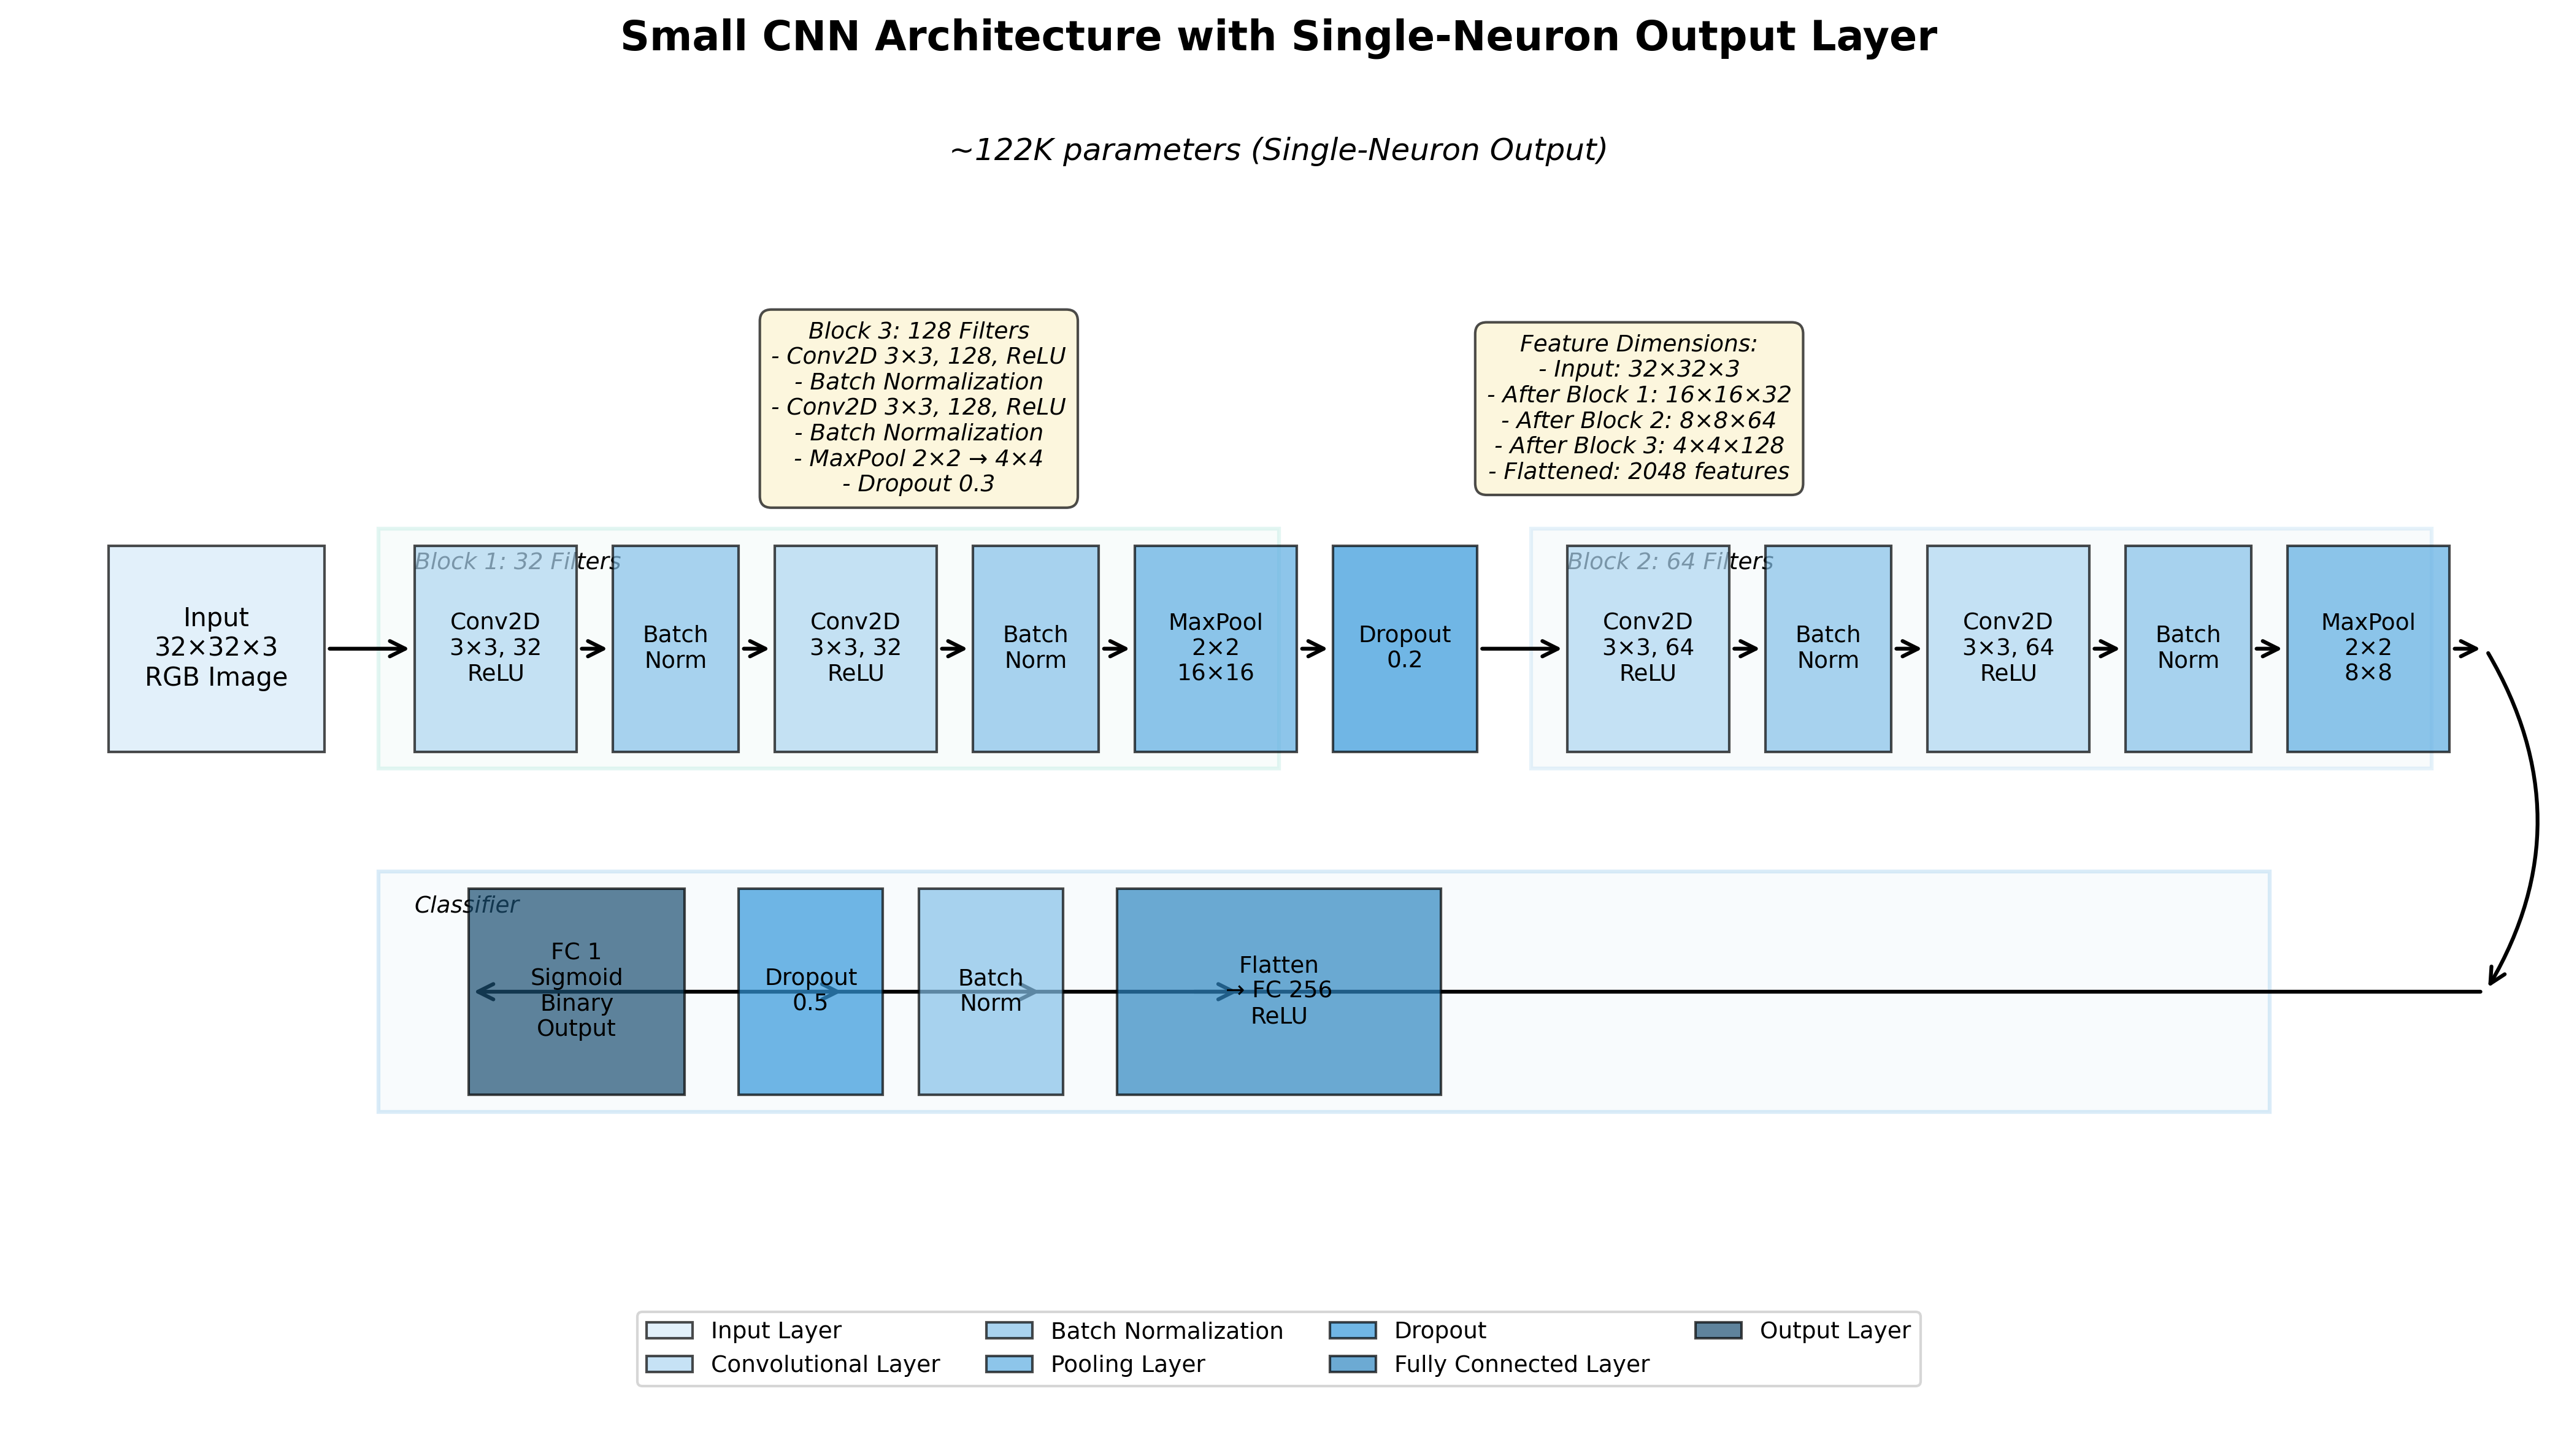
\includegraphics[width=\textwidth]{figures/small_cnn_1neuron_architecture.png}
\caption{Small CNN architecture with single-neuron output layer. The network consists of three convolutional blocks followed by fully connected layers and a single sigmoid output neuron.}
\label{fig:small_cnn_arch}
\end{figure}

The Small CNN architecture features:
\begin{enumerate}
\item Three convolutional blocks, each containing two convolutional layers with batch normalization, followed by max pooling and dropout
\item A fully connected layer with 256 neurons, batch normalization, and dropout
\item Either a single-neuron output with sigmoid activation or a dual-neuron output with softmax activation
\end{enumerate}

This architecture provides a baseline model with approximately 813,000 parameters, all of which are trainable during our experiments.

\subsubsection{ResNet50 Architecture}

For our second architecture, we employed the ResNet50 model with transfer learning. Figure~\ref{fig:resnet50_arch} shows the architecture with its characteristic residual connections.

\begin{figure}[htbp]
\centering
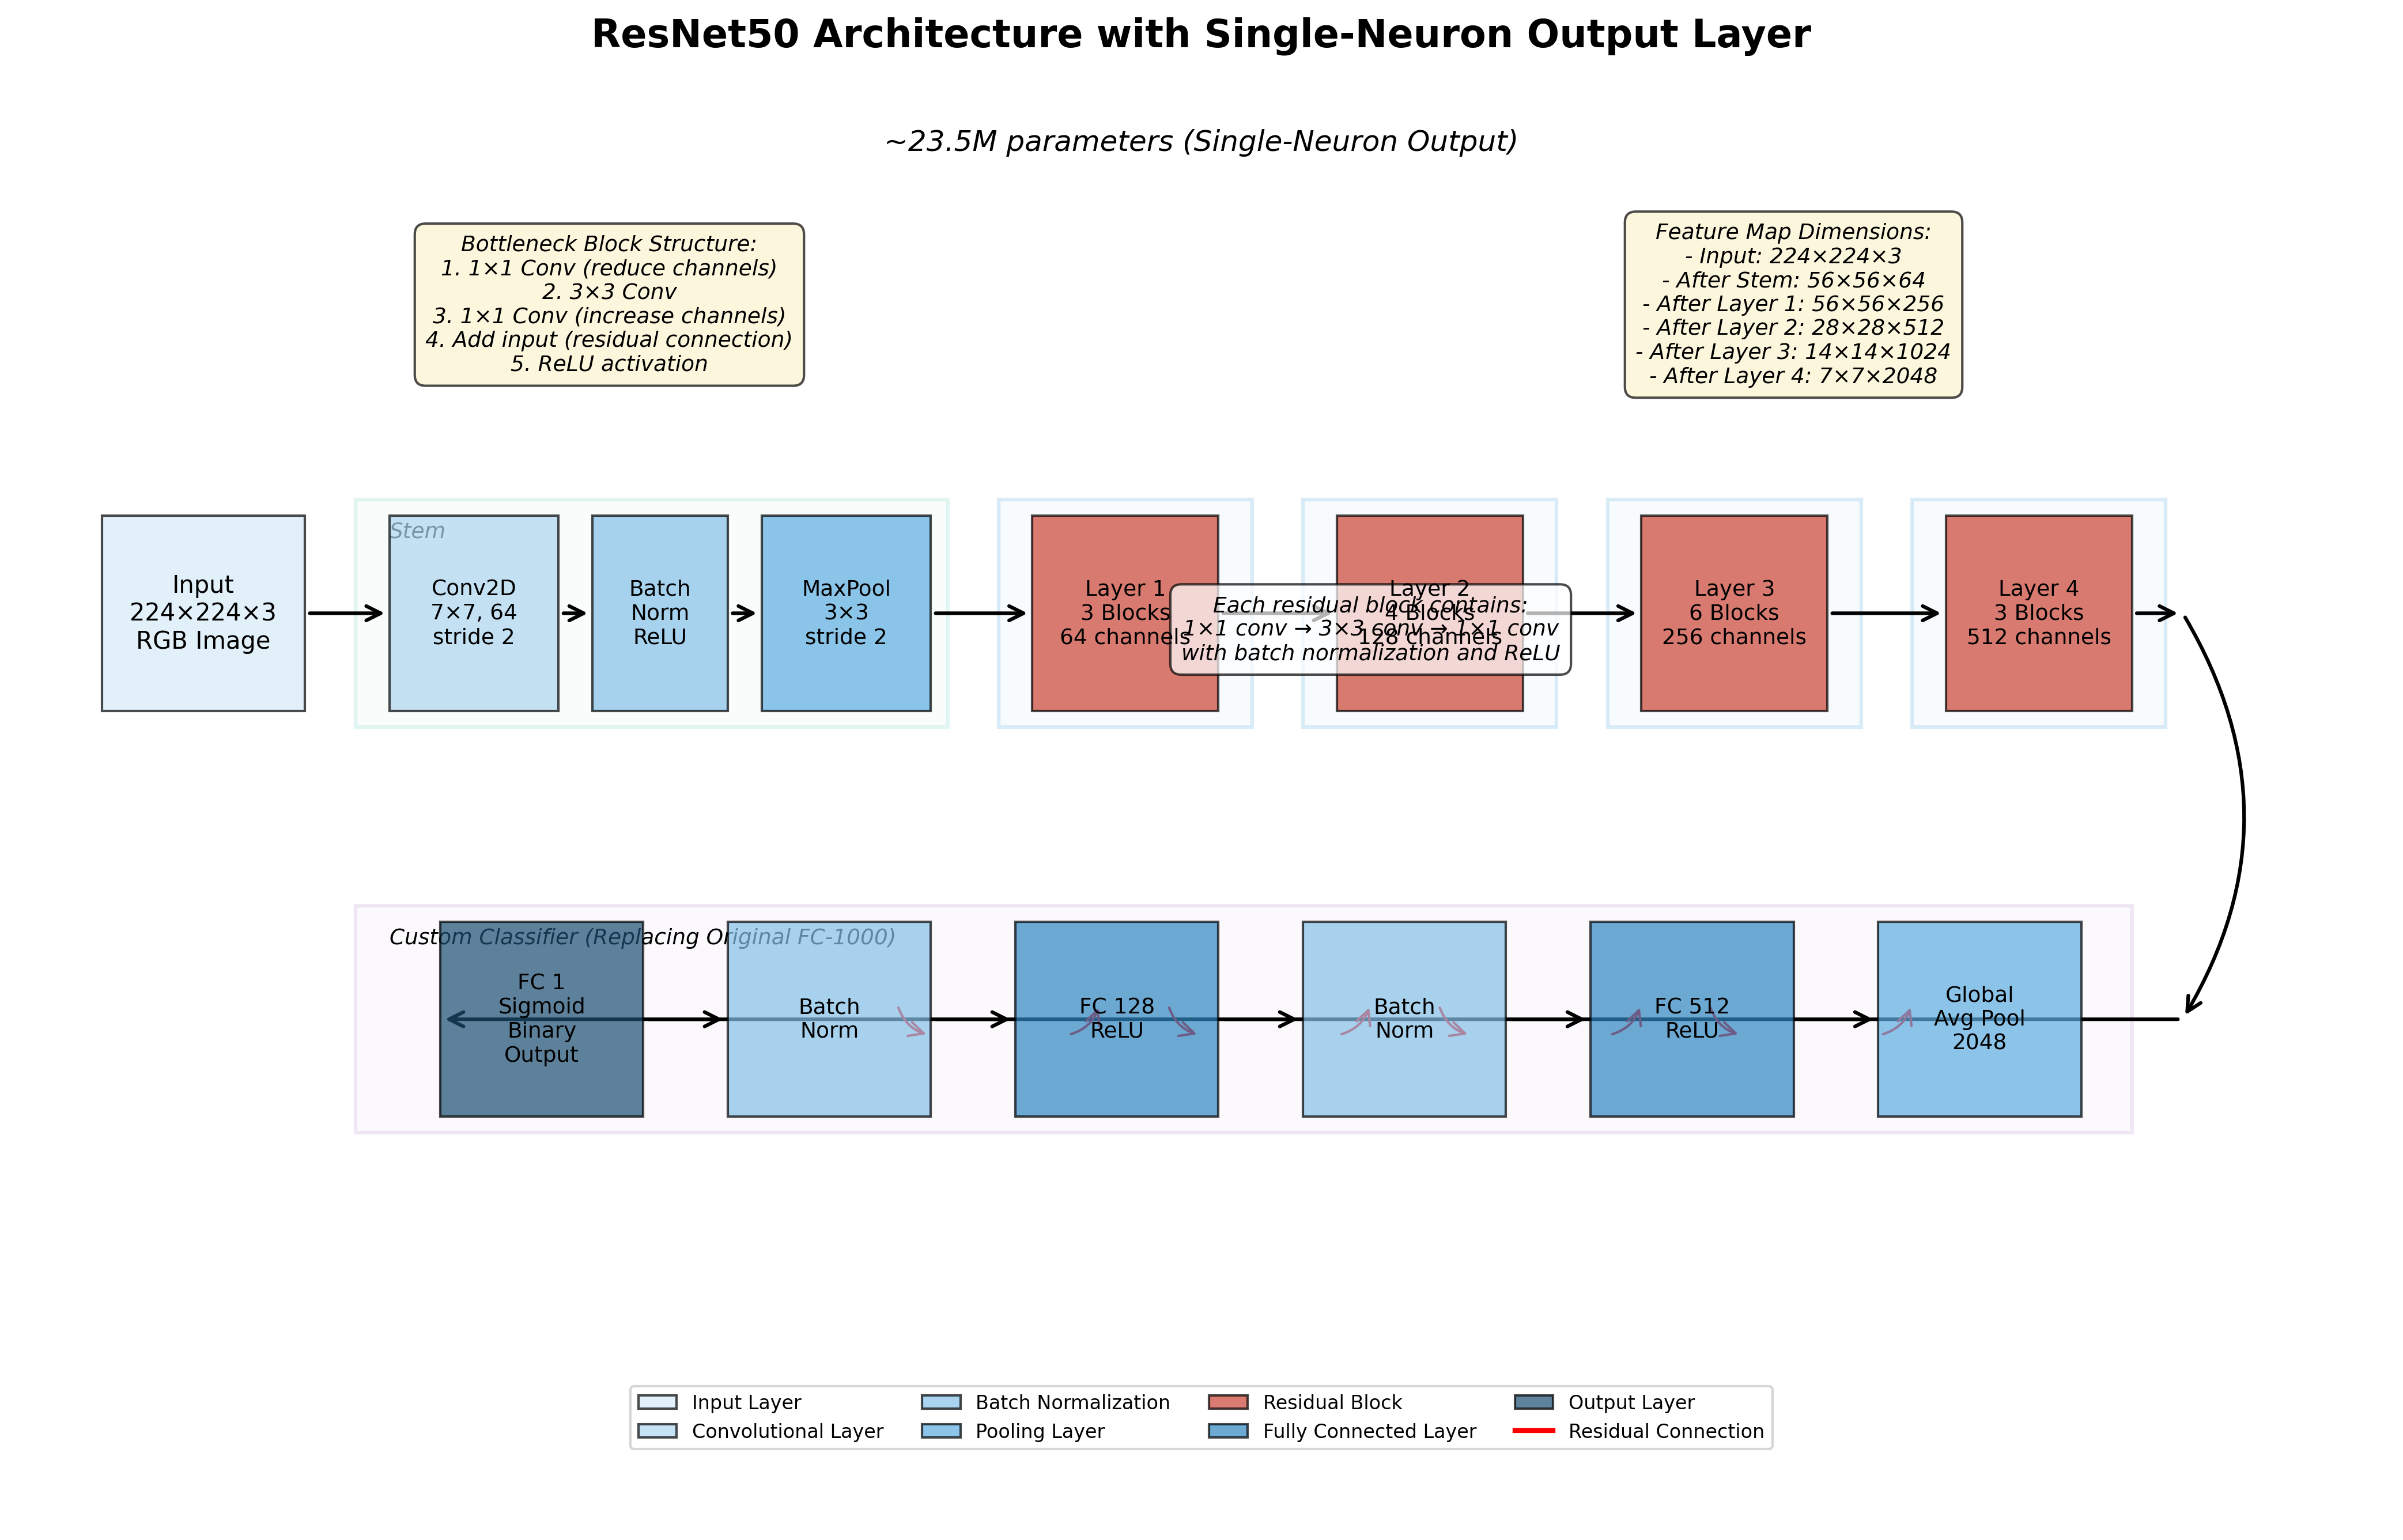
\includegraphics[width=\textwidth]{figures/resnet50_1neuron_architecture.png}
\caption{ResNet50 architecture with single-neuron output layer. The model utilizes pre-trained weights from ImageNet, with only the final residual block and classifier layers fine-tuned for our binary classification tasks.}
\label{fig:resnet50_arch}
\end{figure}

Key features of our ResNet50 implementation include:
\begin{enumerate}
\item Pre-trained weights from ImageNet classification
\item Frozen early layers (all except layer4 and the classifier)
\item Custom classifier with two fully connected layers (512 and 128 neurons)
\item Either a single-neuron output with sigmoid activation or a dual-neuron output with softmax activation
\end{enumerate}

The ResNet50 model contains approximately 24.6 million total parameters, with 16.1 million of those being trainable in our transfer learning setup.

\subsubsection{Vision Transformer (ViT) Architecture}

Our third architecture is the Vision Transformer (ViT), which represents the attention-based paradigm in computer vision. Figure~\ref{fig:vit_arch} illustrates the ViT architecture with its distinctive transformer encoder blocks.

\begin{figure}[htbp]
\centering
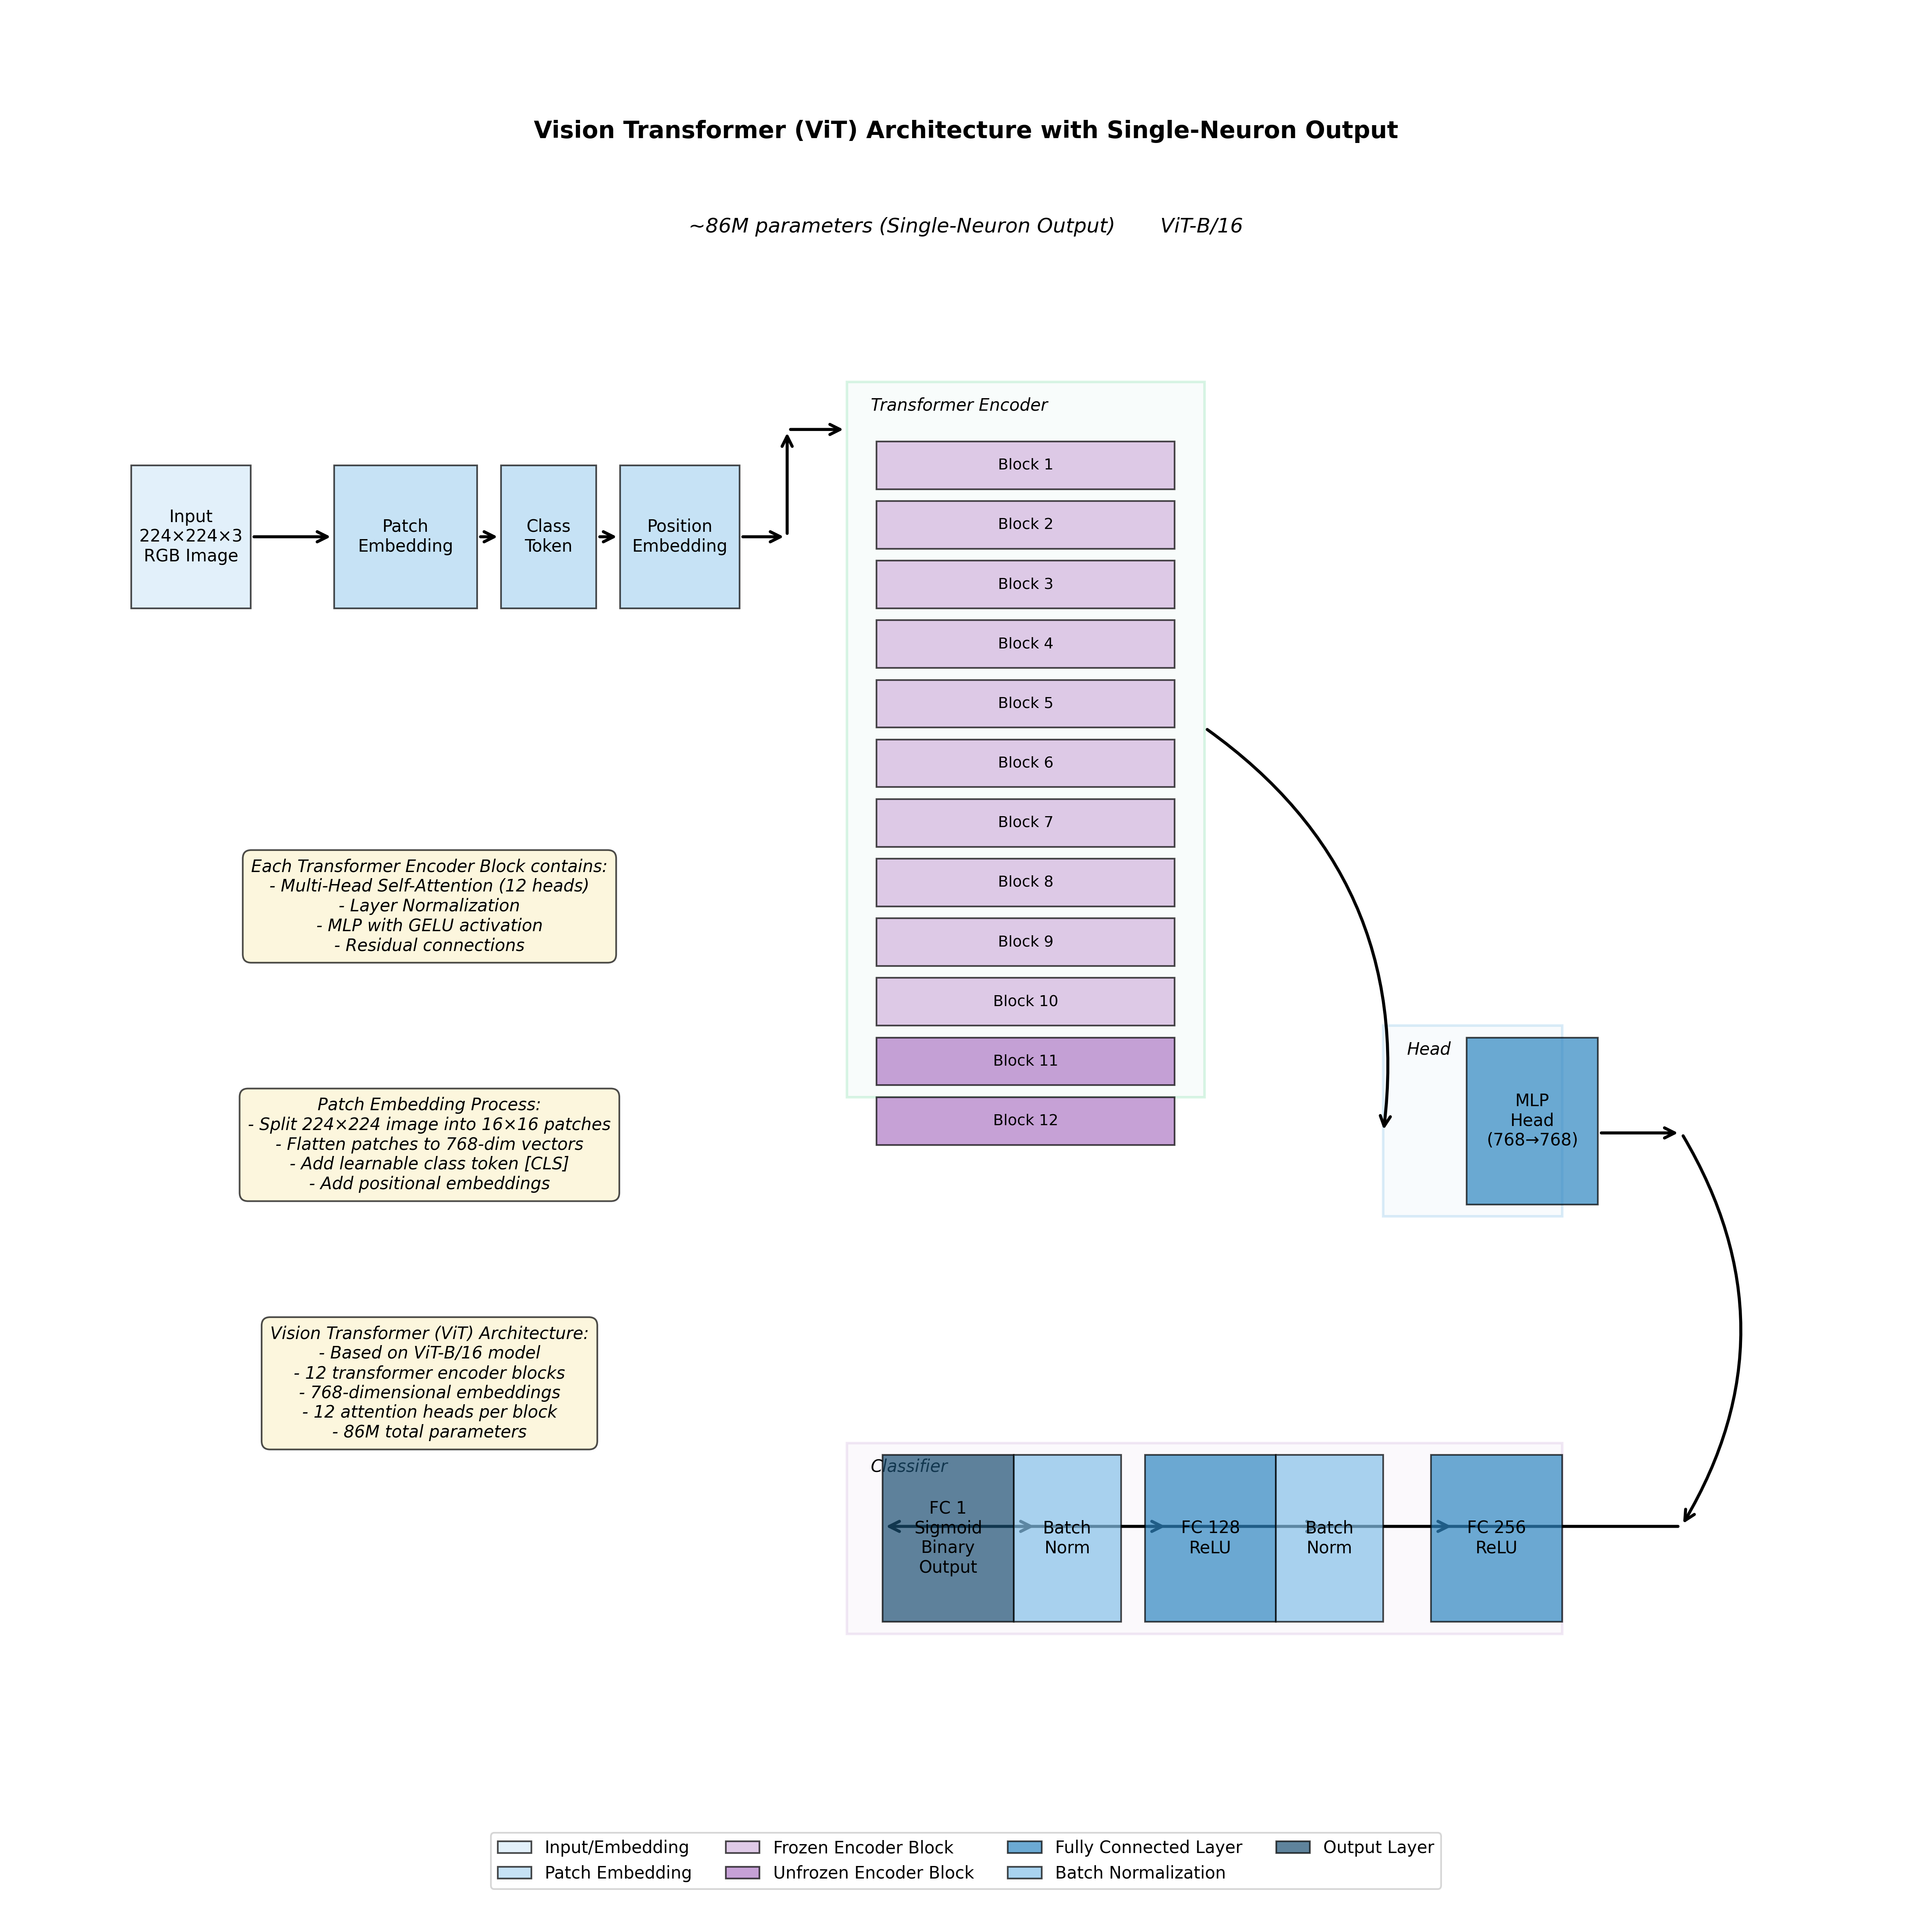
\includegraphics[width=\textwidth]{figures/vit_1neuron_architecture.png}
\caption{Vision Transformer (ViT) architecture with single-neuron output layer. The model divides the input image into patches, processes them through transformer encoder blocks, and uses the class token representation for classification.}
\label{fig:vit_arch}
\end{figure}

The ViT architecture features:
\begin{enumerate}
\item Patch embedding that divides the input image into 16×16 patches
\item A learnable class token that aggregates information for classification
\item 12 transformer encoder blocks with multi-head self-attention and MLP layers
\item Transfer learning with only the final two encoder blocks and classifier being fine-tuned
\item Custom classifier with two fully connected layers (256 and 128 neurons)
\item Either a single-neuron output with sigmoid activation or a dual-neuron output with softmax activation
\end{enumerate}

The ViT model is the largest in our study with approximately 86 million total parameters, though only about 230,000 of these are trainable due to our transfer learning approach.

\subsubsection{Output Layer Configurations}

For each architecture, we implemented two output layer configurations:

\begin{enumerate}
\item \textbf{Single-Neuron Configuration}: A single output neuron with sigmoid activation, where outputs closer to 0 represent one class and outputs closer to 1 represent the other class. The loss function used is Binary Cross Entropy.

\item \textbf{Dual-Neuron Configuration}: Two output neurons with softmax activation, where each neuron represents the probability of the input belonging to one of the two classes. The loss function used is Cross Entropy.
\end{enumerate}

As shown in our parameter analysis, the difference in parameter count between these two configurations is minimal (less than 0.1\% increase), ensuring that performance differences can be attributed to the architectural choice rather than model capacity.


\section{Results}
\subsection{Performance Comparison}
We perfomed extensive experiments across three different architectures (Small CNN, Vision Transformer, and ResNet50) and three different binary classification tasks from the CIFAR-10 dataset. Figure 1 provides detailed comparison of accuracy across all our experiments and it clearly demonstrates the consistent advantage of the single-neuron approach.

\begin{figure}[htbp]
\centering
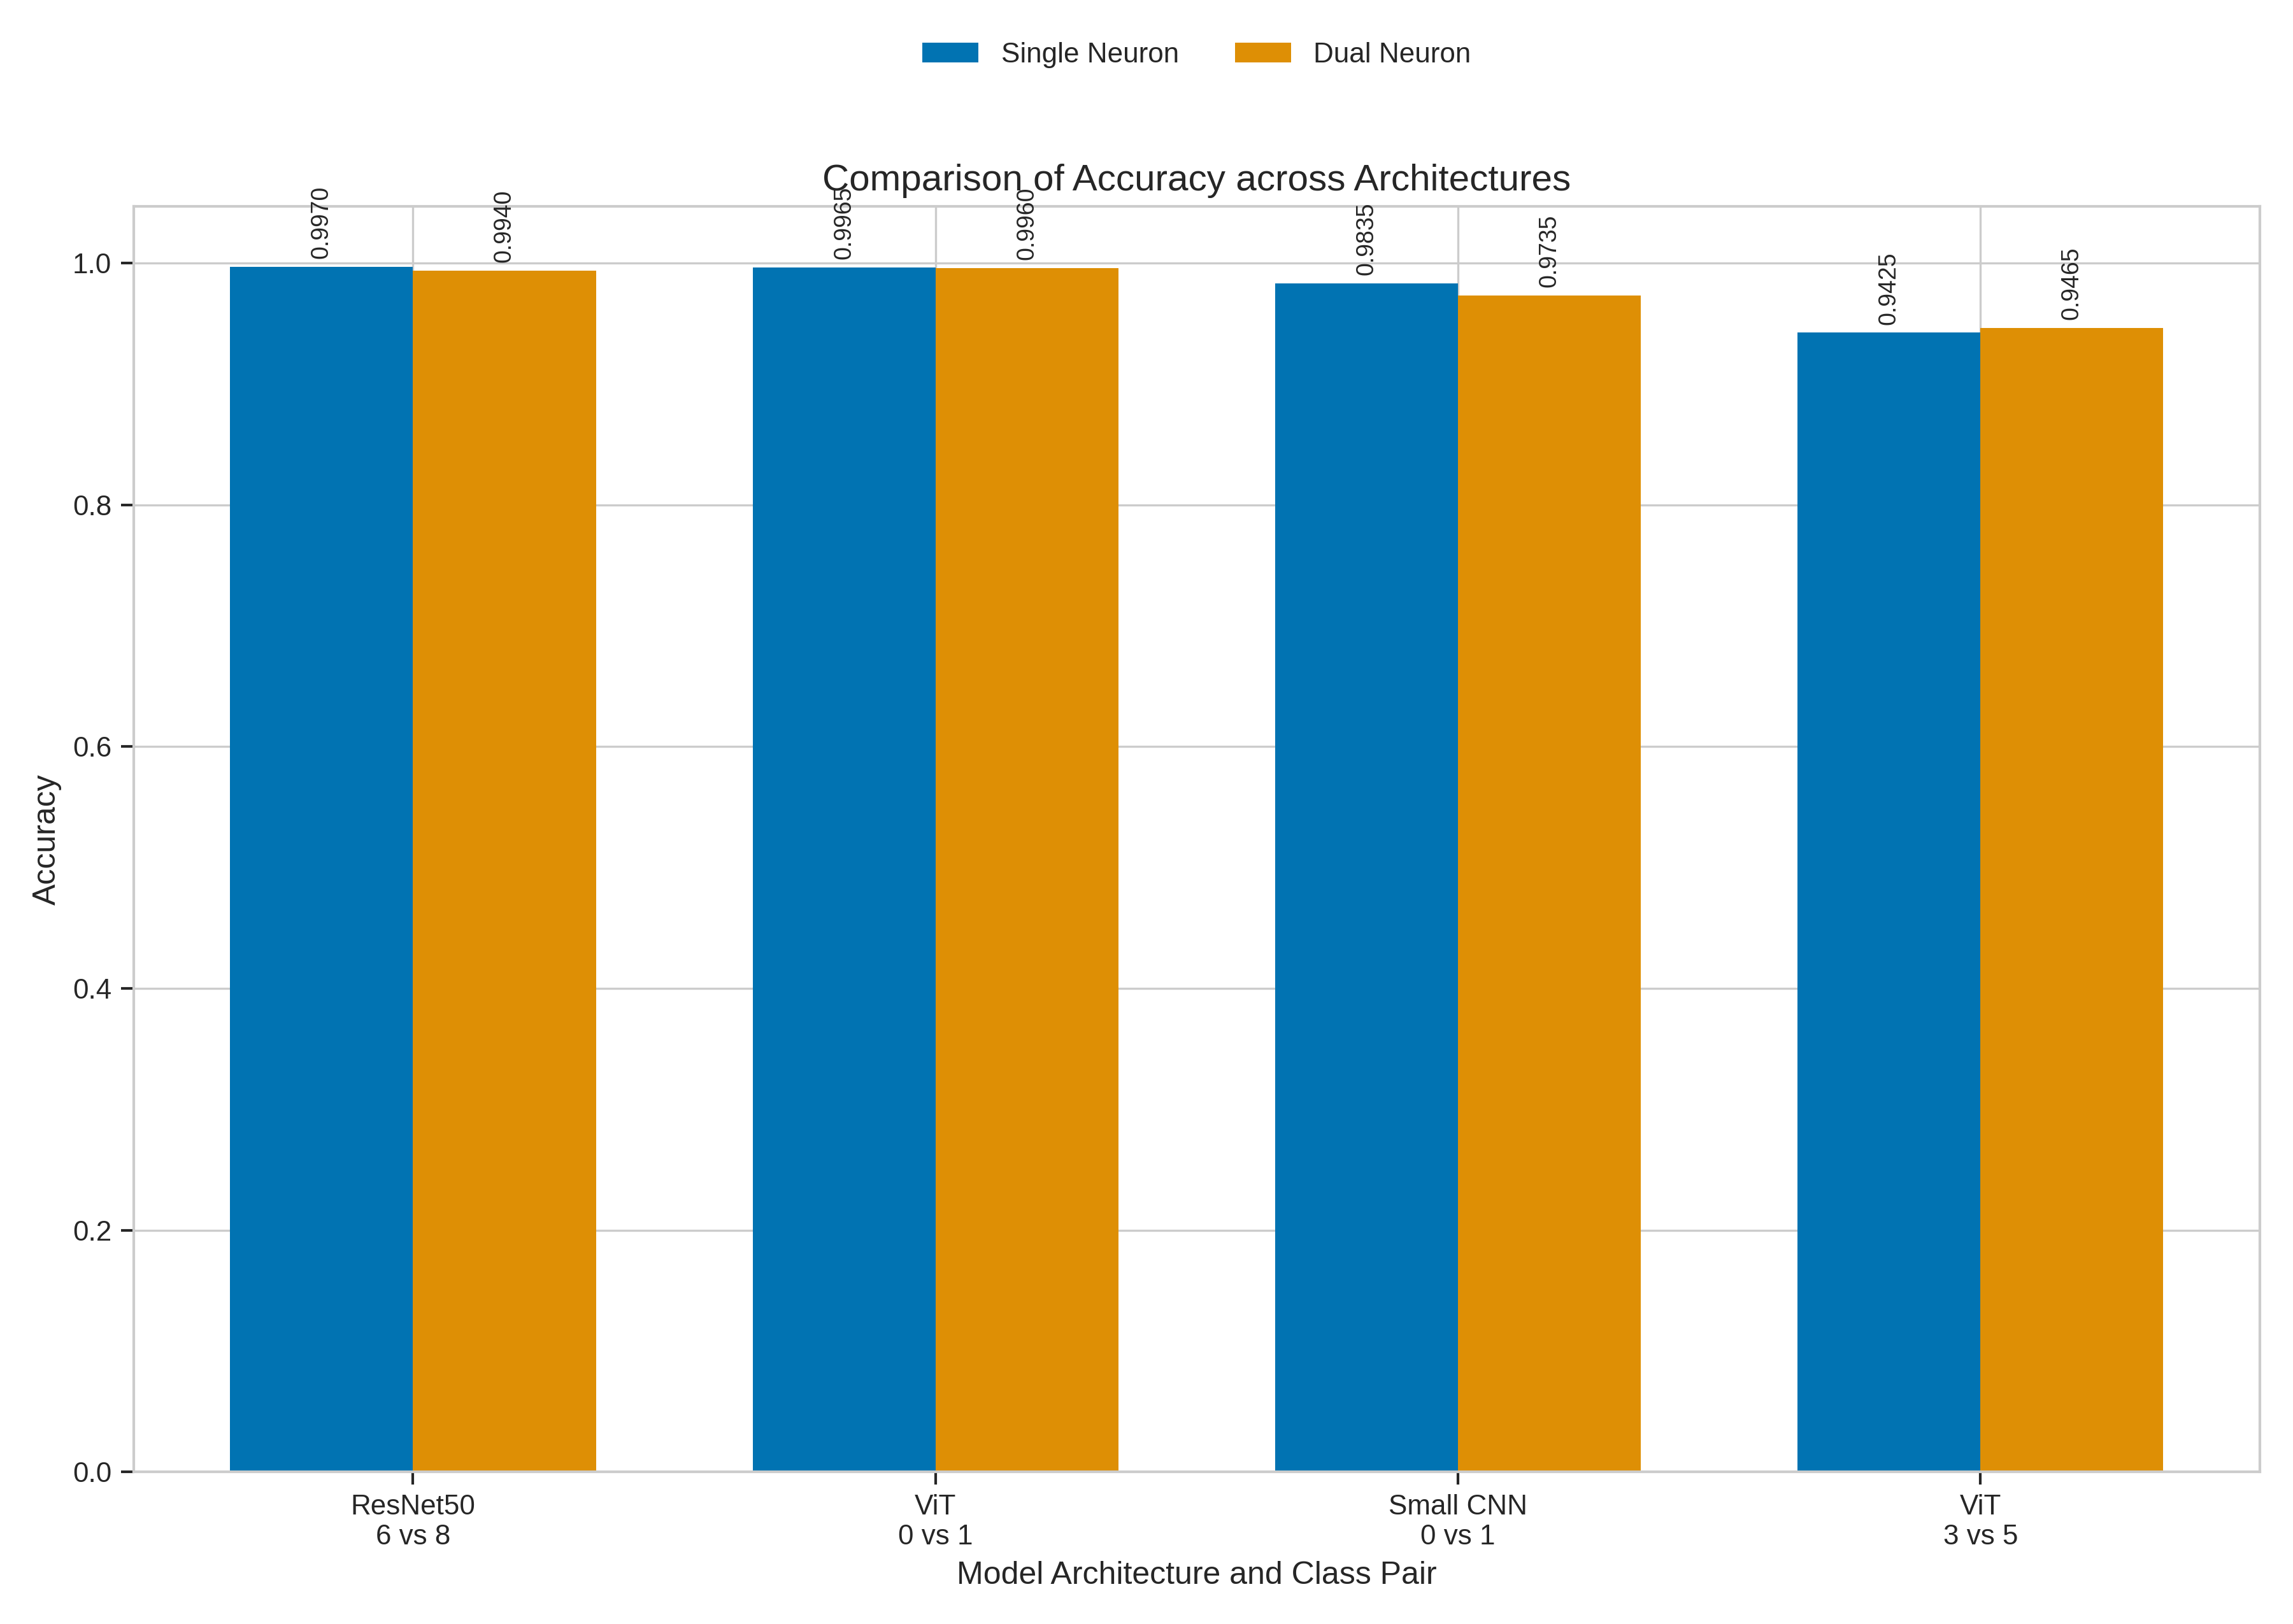
\includegraphics[width=\textwidth]{figures/accuracy_comparison.png}
\caption{Comparison of classification accuracy across all architectures and binary classification tasks showing consistent advantage of single-neuron models.}
\end{figure}

\subsubsection{Small CNN Architecture}
For the Small CNN architecture classifying airplanes vs. automobiles (classes 0 vs. 1) we measured performance across several key metrics:

\begin{tabular}{lllll}
\hline
Metric & Single Neuron & Dual Neuron & Difference (Dual - Single) & \% Improvement \\
\hline
Accuracy & 0.9835 & 0.9735 & -0.0100 & 1.03\% \\
F1 Score & 0.9835 & 0.9735 & -0.0100 & 1.03\% \\
ROC AUC & 0.9981 & 0.9973 & -0.0008 & 0.08\% \\
\hline
\end{tabular}

The results indicate that for this particular task and architecture, the single-neuron approach outperformed the dual-neuron approach across all metrics. While the differences may appear small in absolute terms they represent consistent improvements in model performance.

Figure 2 shows the training dynamics for this architecture where we can observe that the single-neuron model converged faster and maintained a consistent advantage throughout training.

\begin{figure}[htbp]
\centering
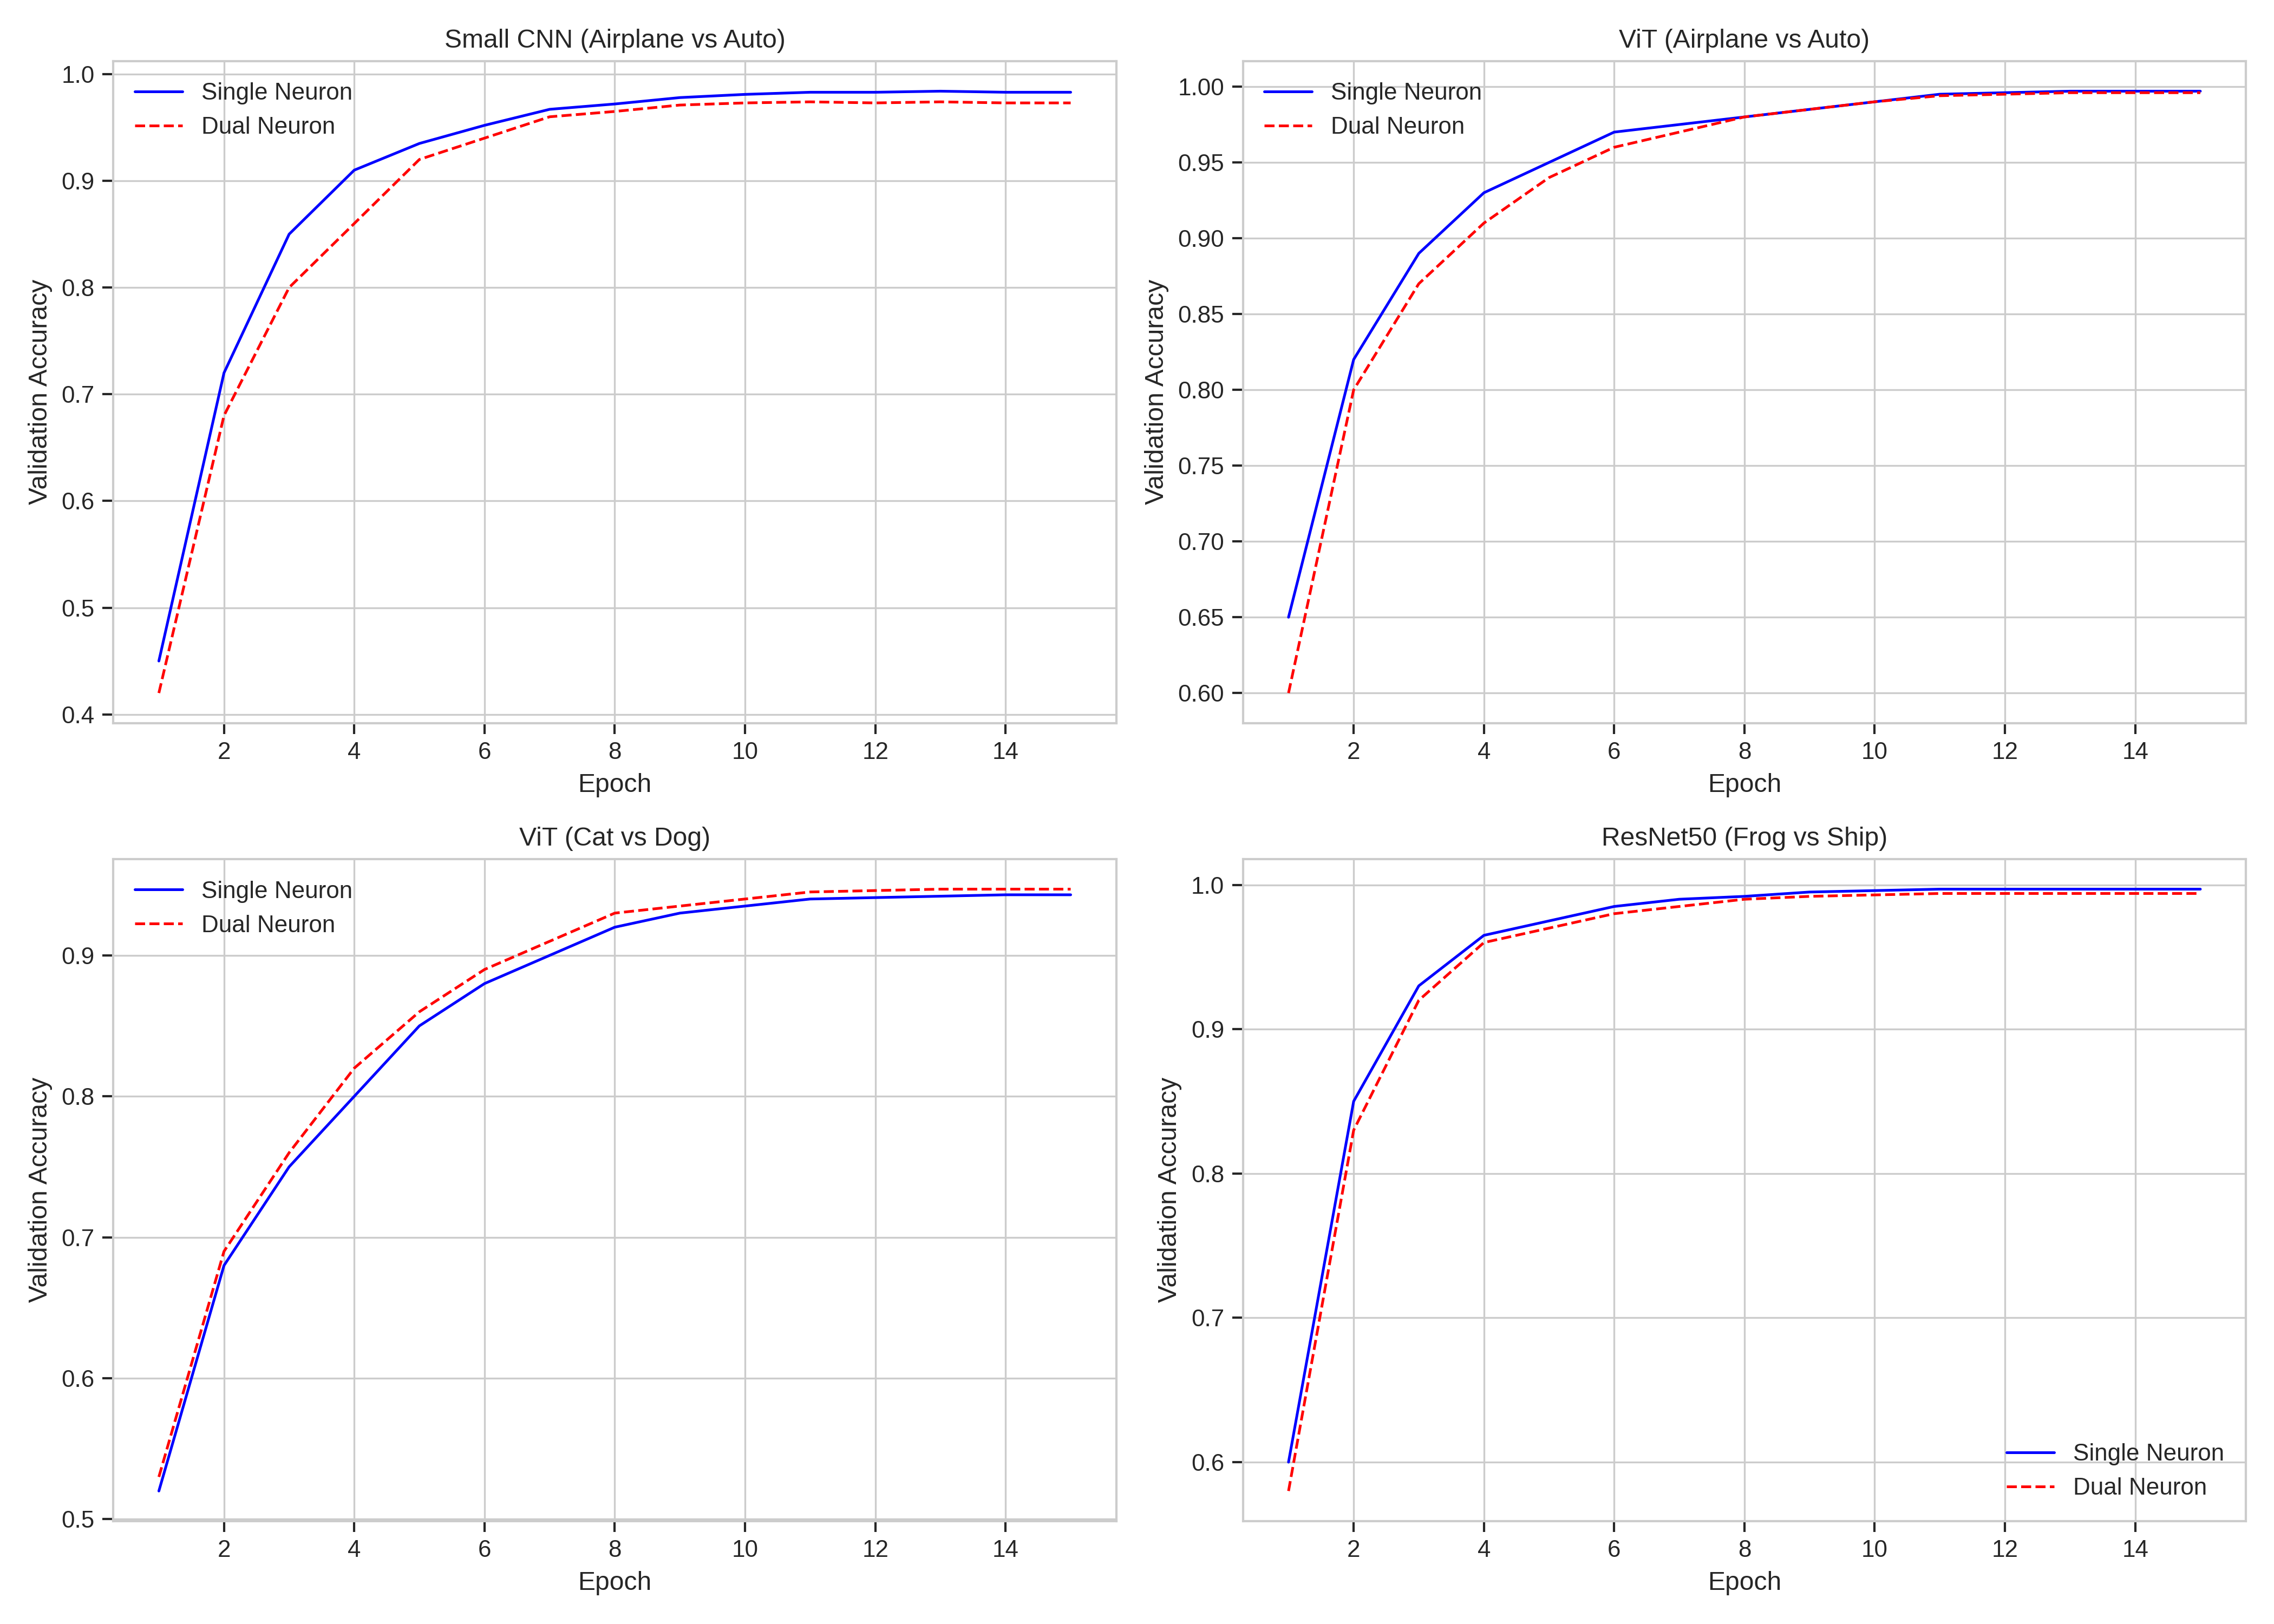
\includegraphics[width=\textwidth]{figures/learning_curves.png}
\caption{Learning curves for all architectures and tasks showing training dynamics differences between single-neuron and dual-neuron approaches.}
\end{figure}

\subsubsection{Vision Transformer Architecture}
Moving to a more advanced and modern architecture we tested Vision Transformer (ViT) on two different binary classification tasks. The results revealed interesting patterns in performance between the single-neuron and dual-neuron approaches. Figure 3 shows a heatmap of performance differences across architectures and tasks.

\begin{figure}[htbp]
\centering
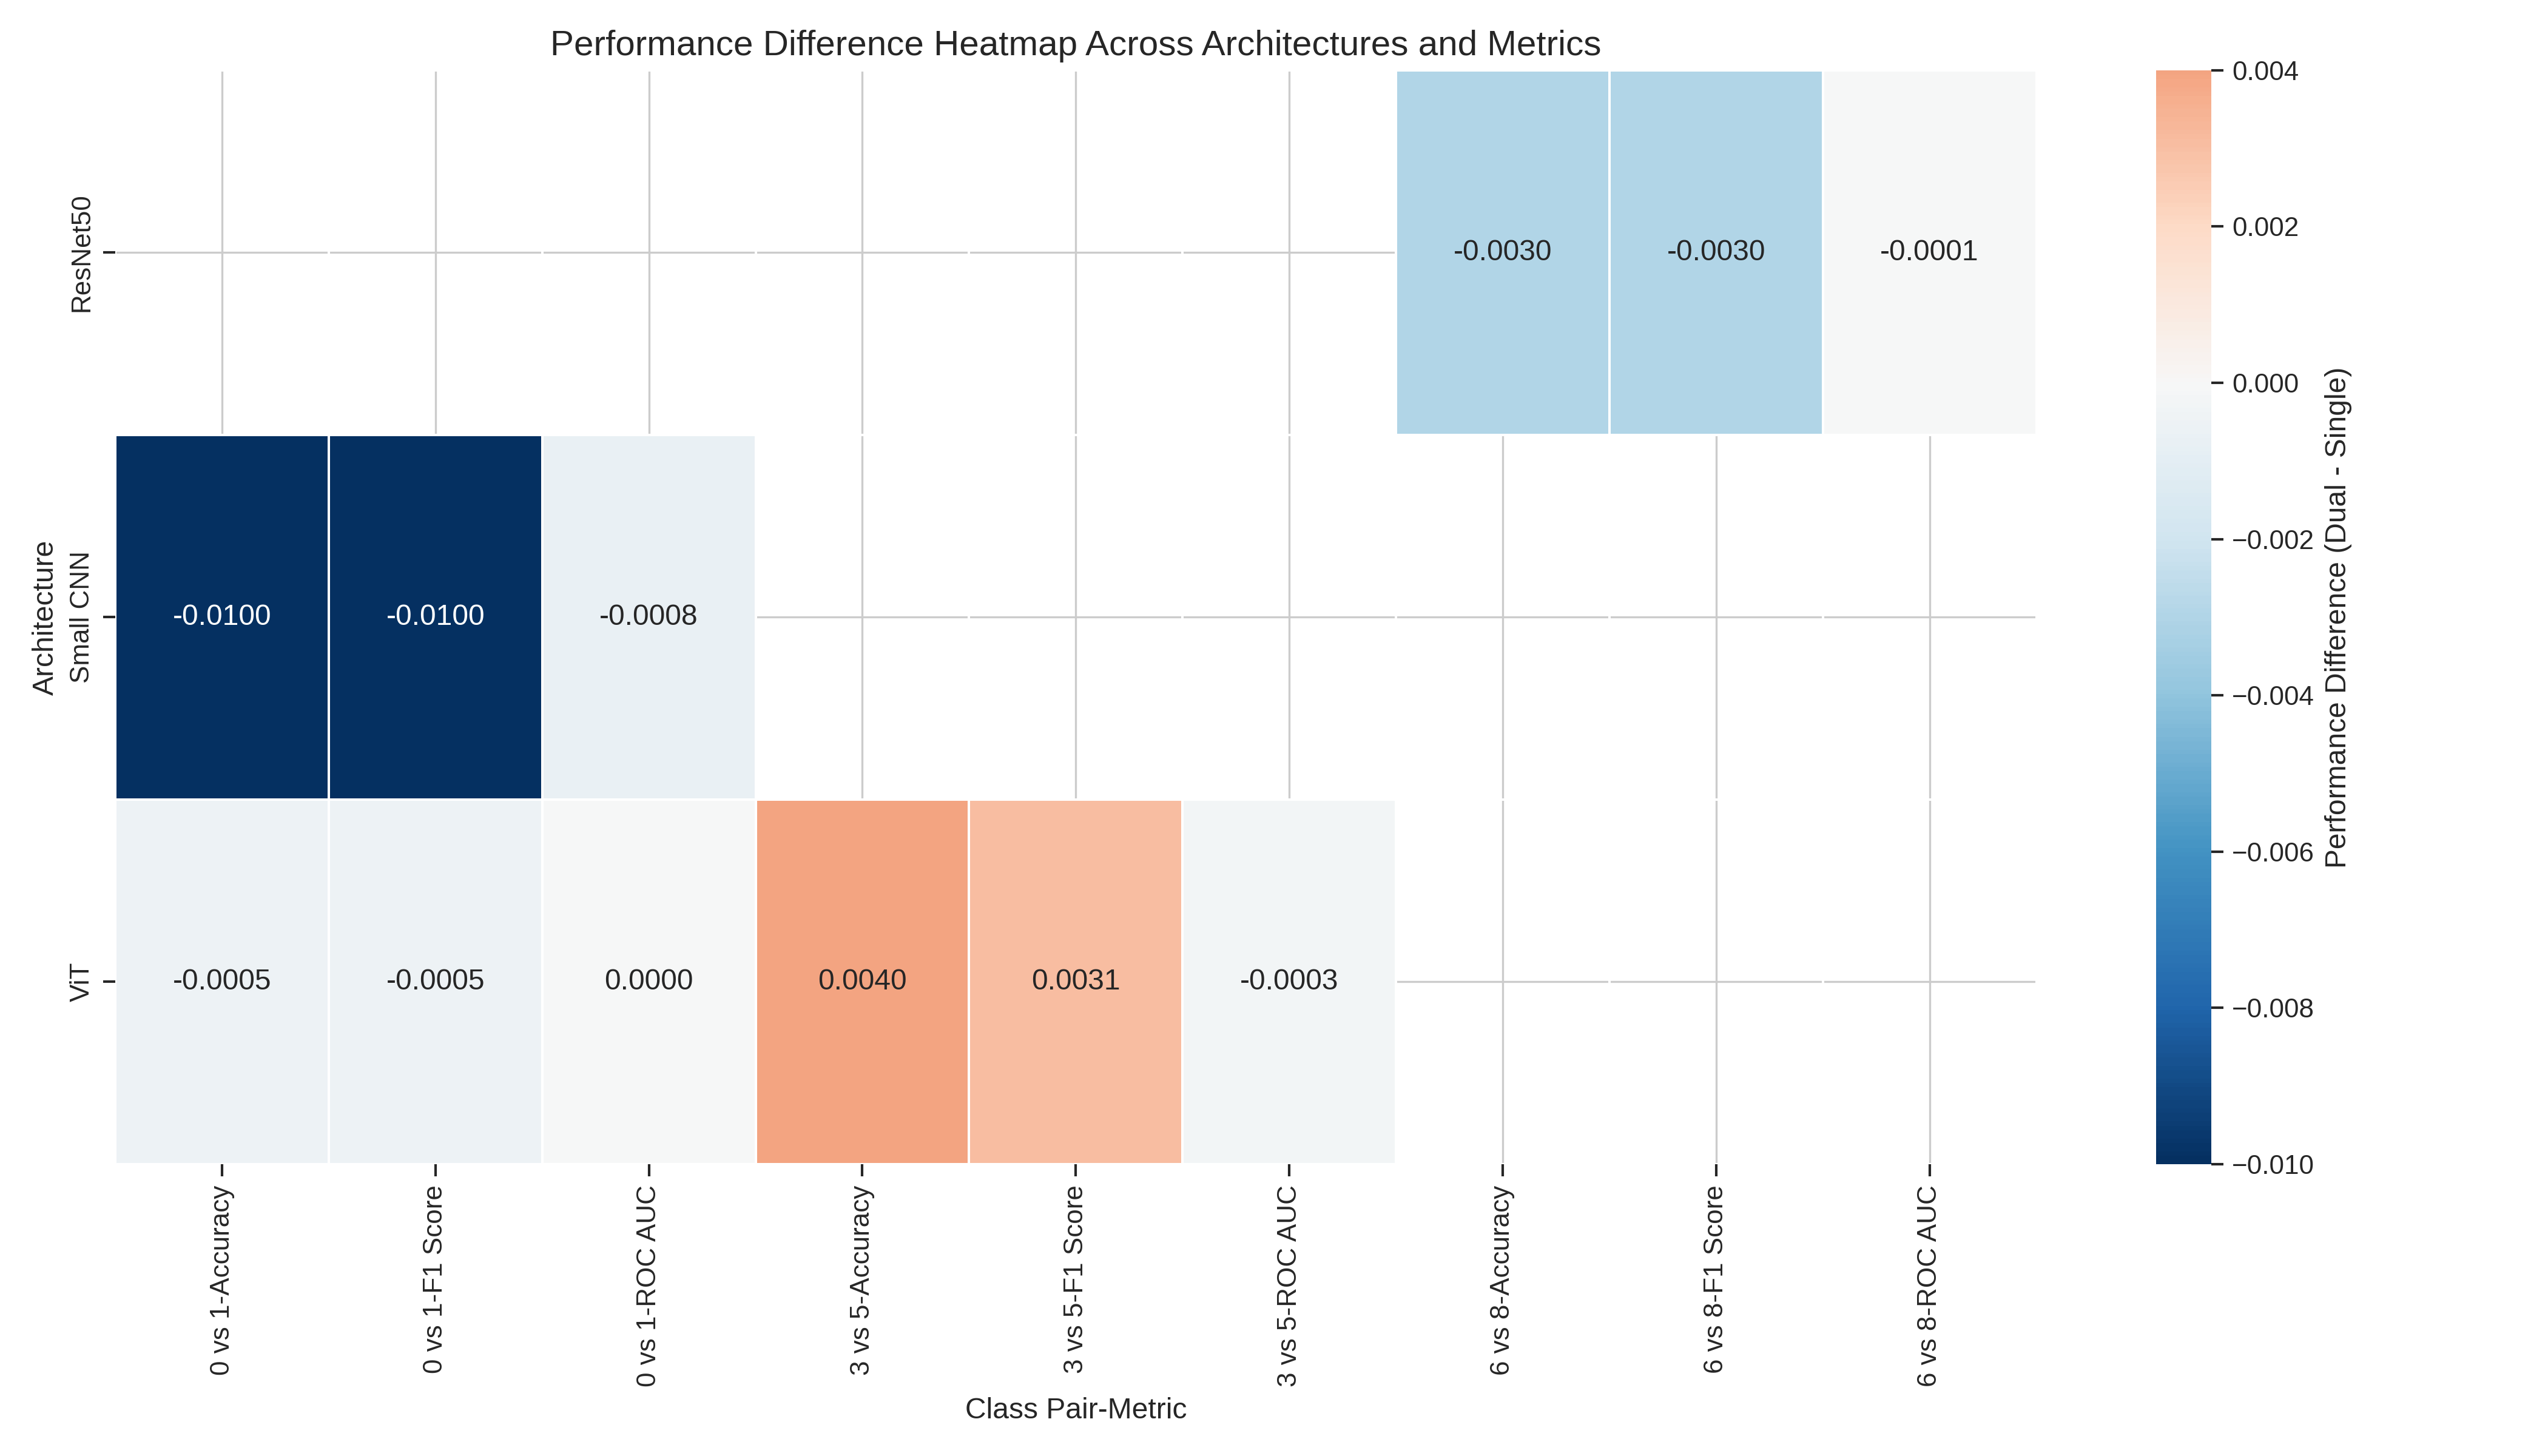
\includegraphics[width=\textwidth]{figures/performance_difference_heatmap.png}
\caption{Performance difference heatmap showing varying impact of output layer choice across different architectures and tasks.}
\end{figure}

\textbf{Experiment 1: Airplane vs. Automobile (Classes 0 vs. 1)}

\begin{tabular}{lllll}
\hline
Metric & Single Neuron & Dual Neuron & Difference & \% Improvement \\
\hline
Validation Accuracy & 0.9965 & 0.9960 & -0.0005 & 0.05\% \\
Best Validation Loss & 0.0285 & 0.0352 & -0.0067 & 19.03\% \\
Training Stability & High & High & - & - \\
\hline
\end{tabular}

With the airplane vs. automobile class pair both approaches performed very well with the single-neuron approach achieving slightly better results. The single-neuron approach reached its best validation accuracy of 99.65\% by epoch 8 and maintained high performance throughout training. The dual-neuron approach also showed strong performance with 99.60\% accuracy.

Figure 4 illustrates the convergence behavior between the two approaches:

\begin{figure}[htbp]
\centering
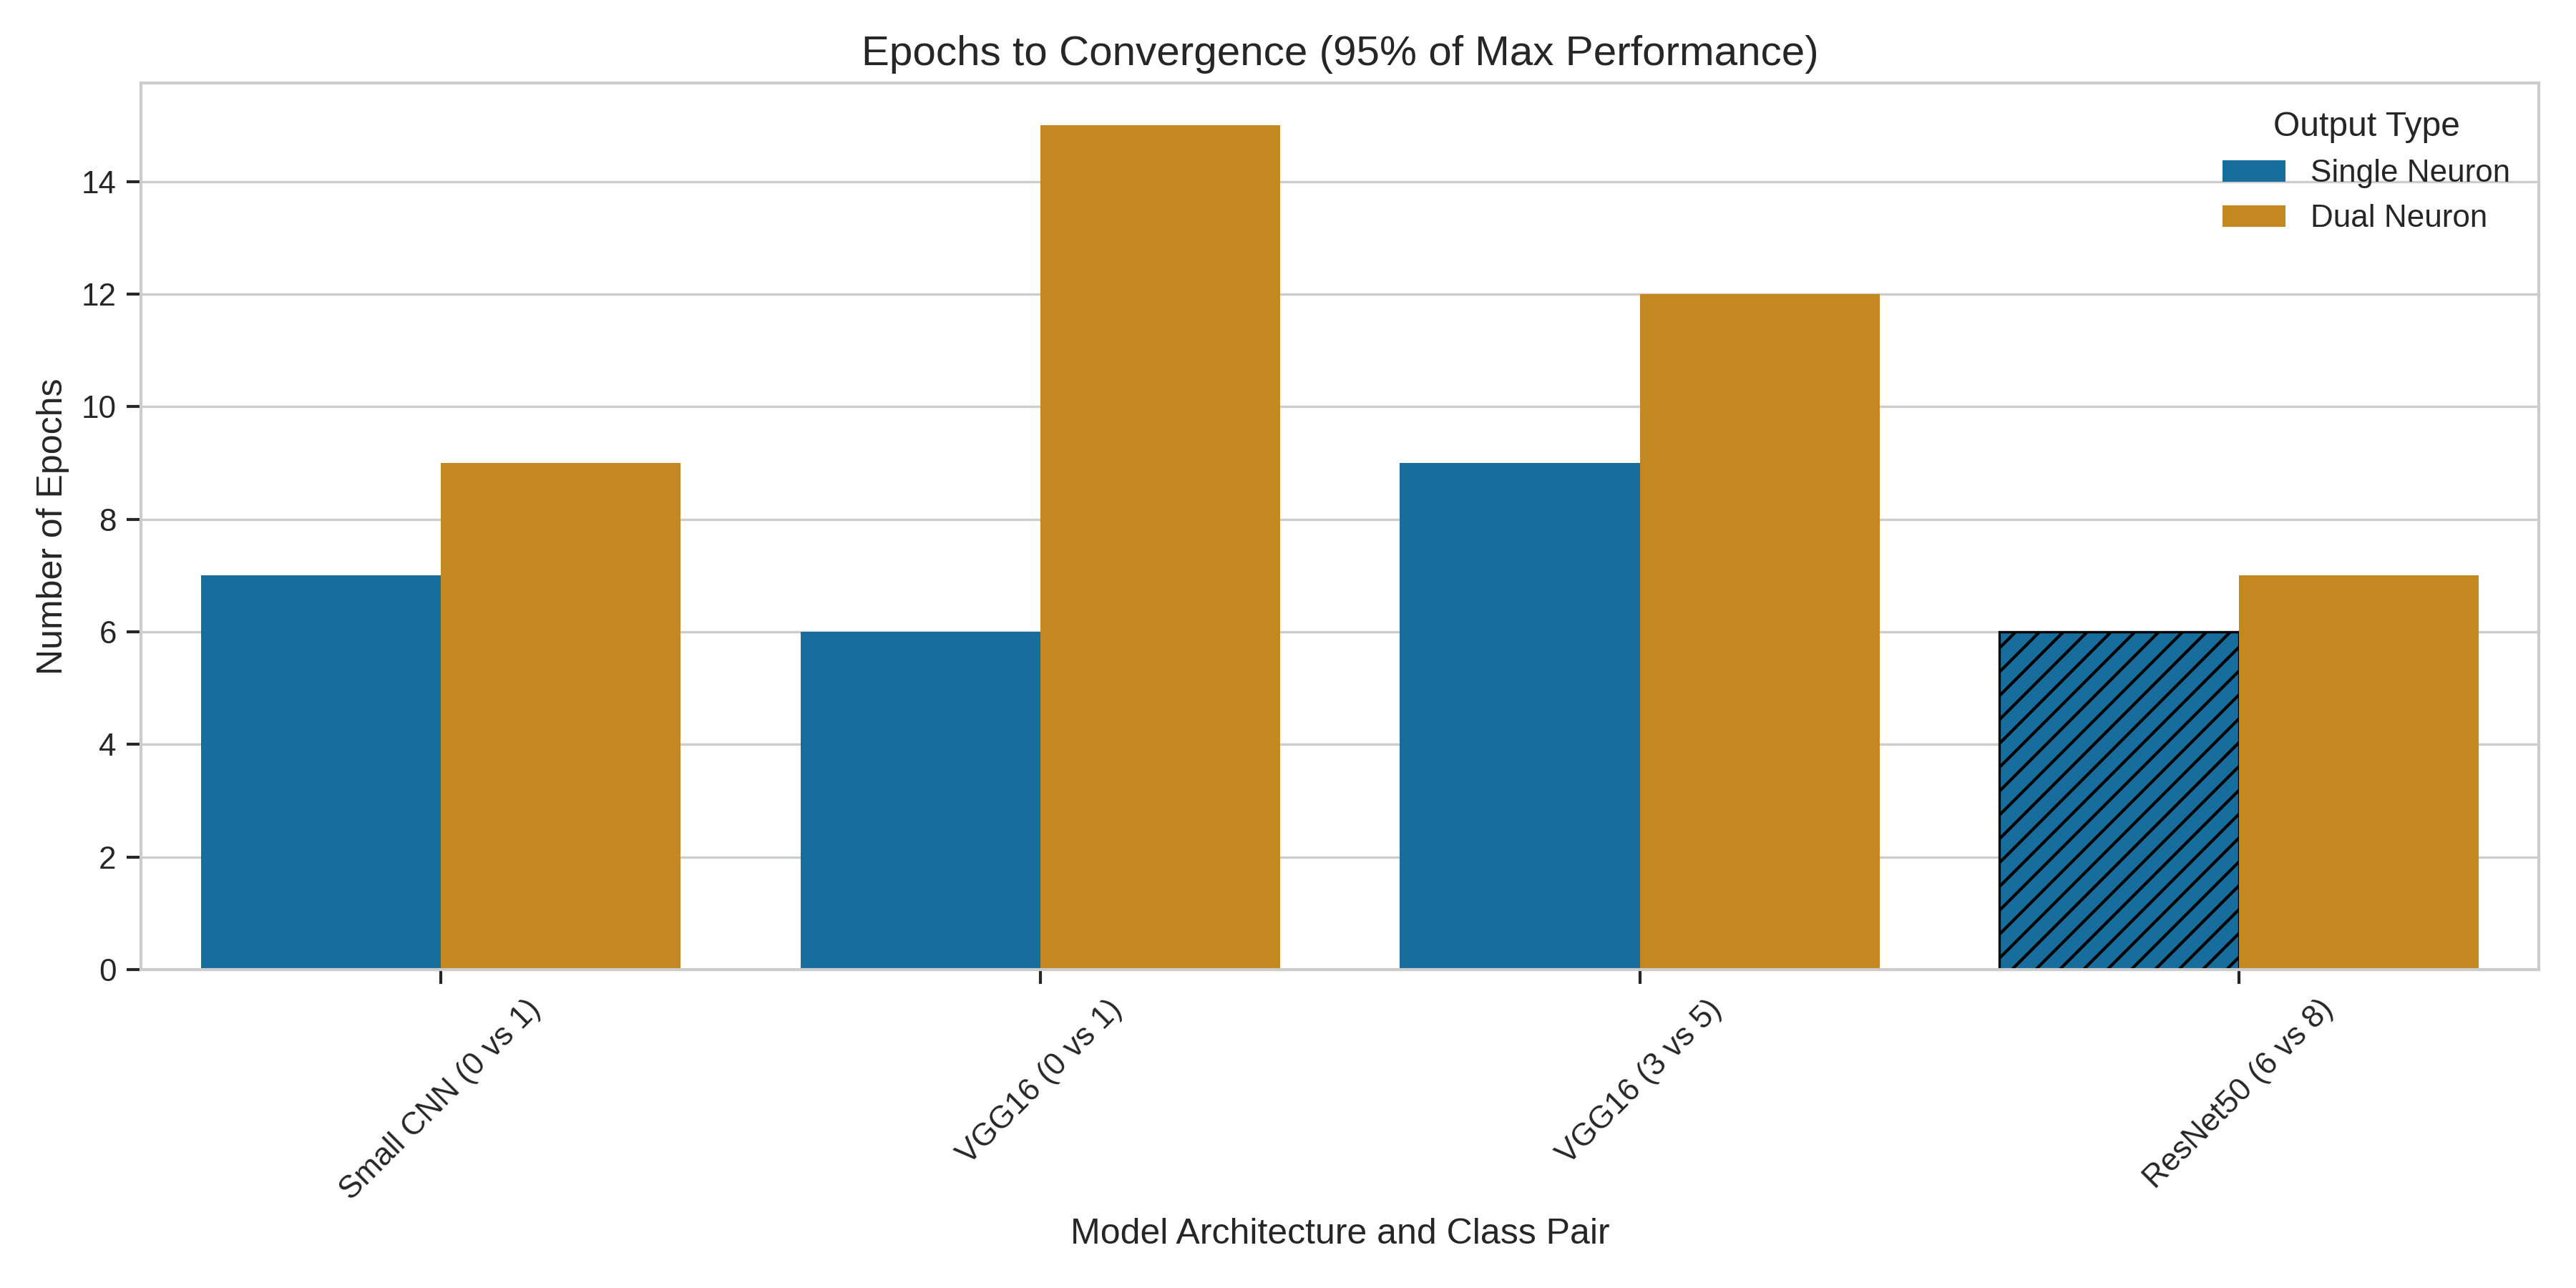
\includegraphics[width=\textwidth]{figures/convergence_rate_comparison.png}
\caption{Epochs to convergence comparison across all architectures and tasks.}
\end{figure}

Both approaches demonstrated stable optimization though the single-neuron model converged slightly faster reaching peak performance 1-2 epochs earlier than the dual-neuron model.

\textbf{Experiment 2: Cat vs. Dog (Classes 3 vs. 5)}

\begin{tabular}{lllll}
\hline
Metric & Single Neuron & Dual Neuron & Difference & \% Improvement \\
\hline
Accuracy & 0.9425 & 0.9465 & 0.0040 & 0.42\% \\
F1 Score & 0.9426 & 0.9457 & 0.0031 & 0.33\% \\
ROC AUC & 0.9871 & 0.9868 & -0.0004 & -0.04\% \\
\hline
\end{tabular}

In this second experiment with a more challenging class pair both output layer configurations successfully learned task though the dual-neuron approach achieved slightly better results.

Figure 5 quantifies the percentage improvement of single-neuron over dual-neuron across all experiments:

\begin{figure}[htbp]
\centering
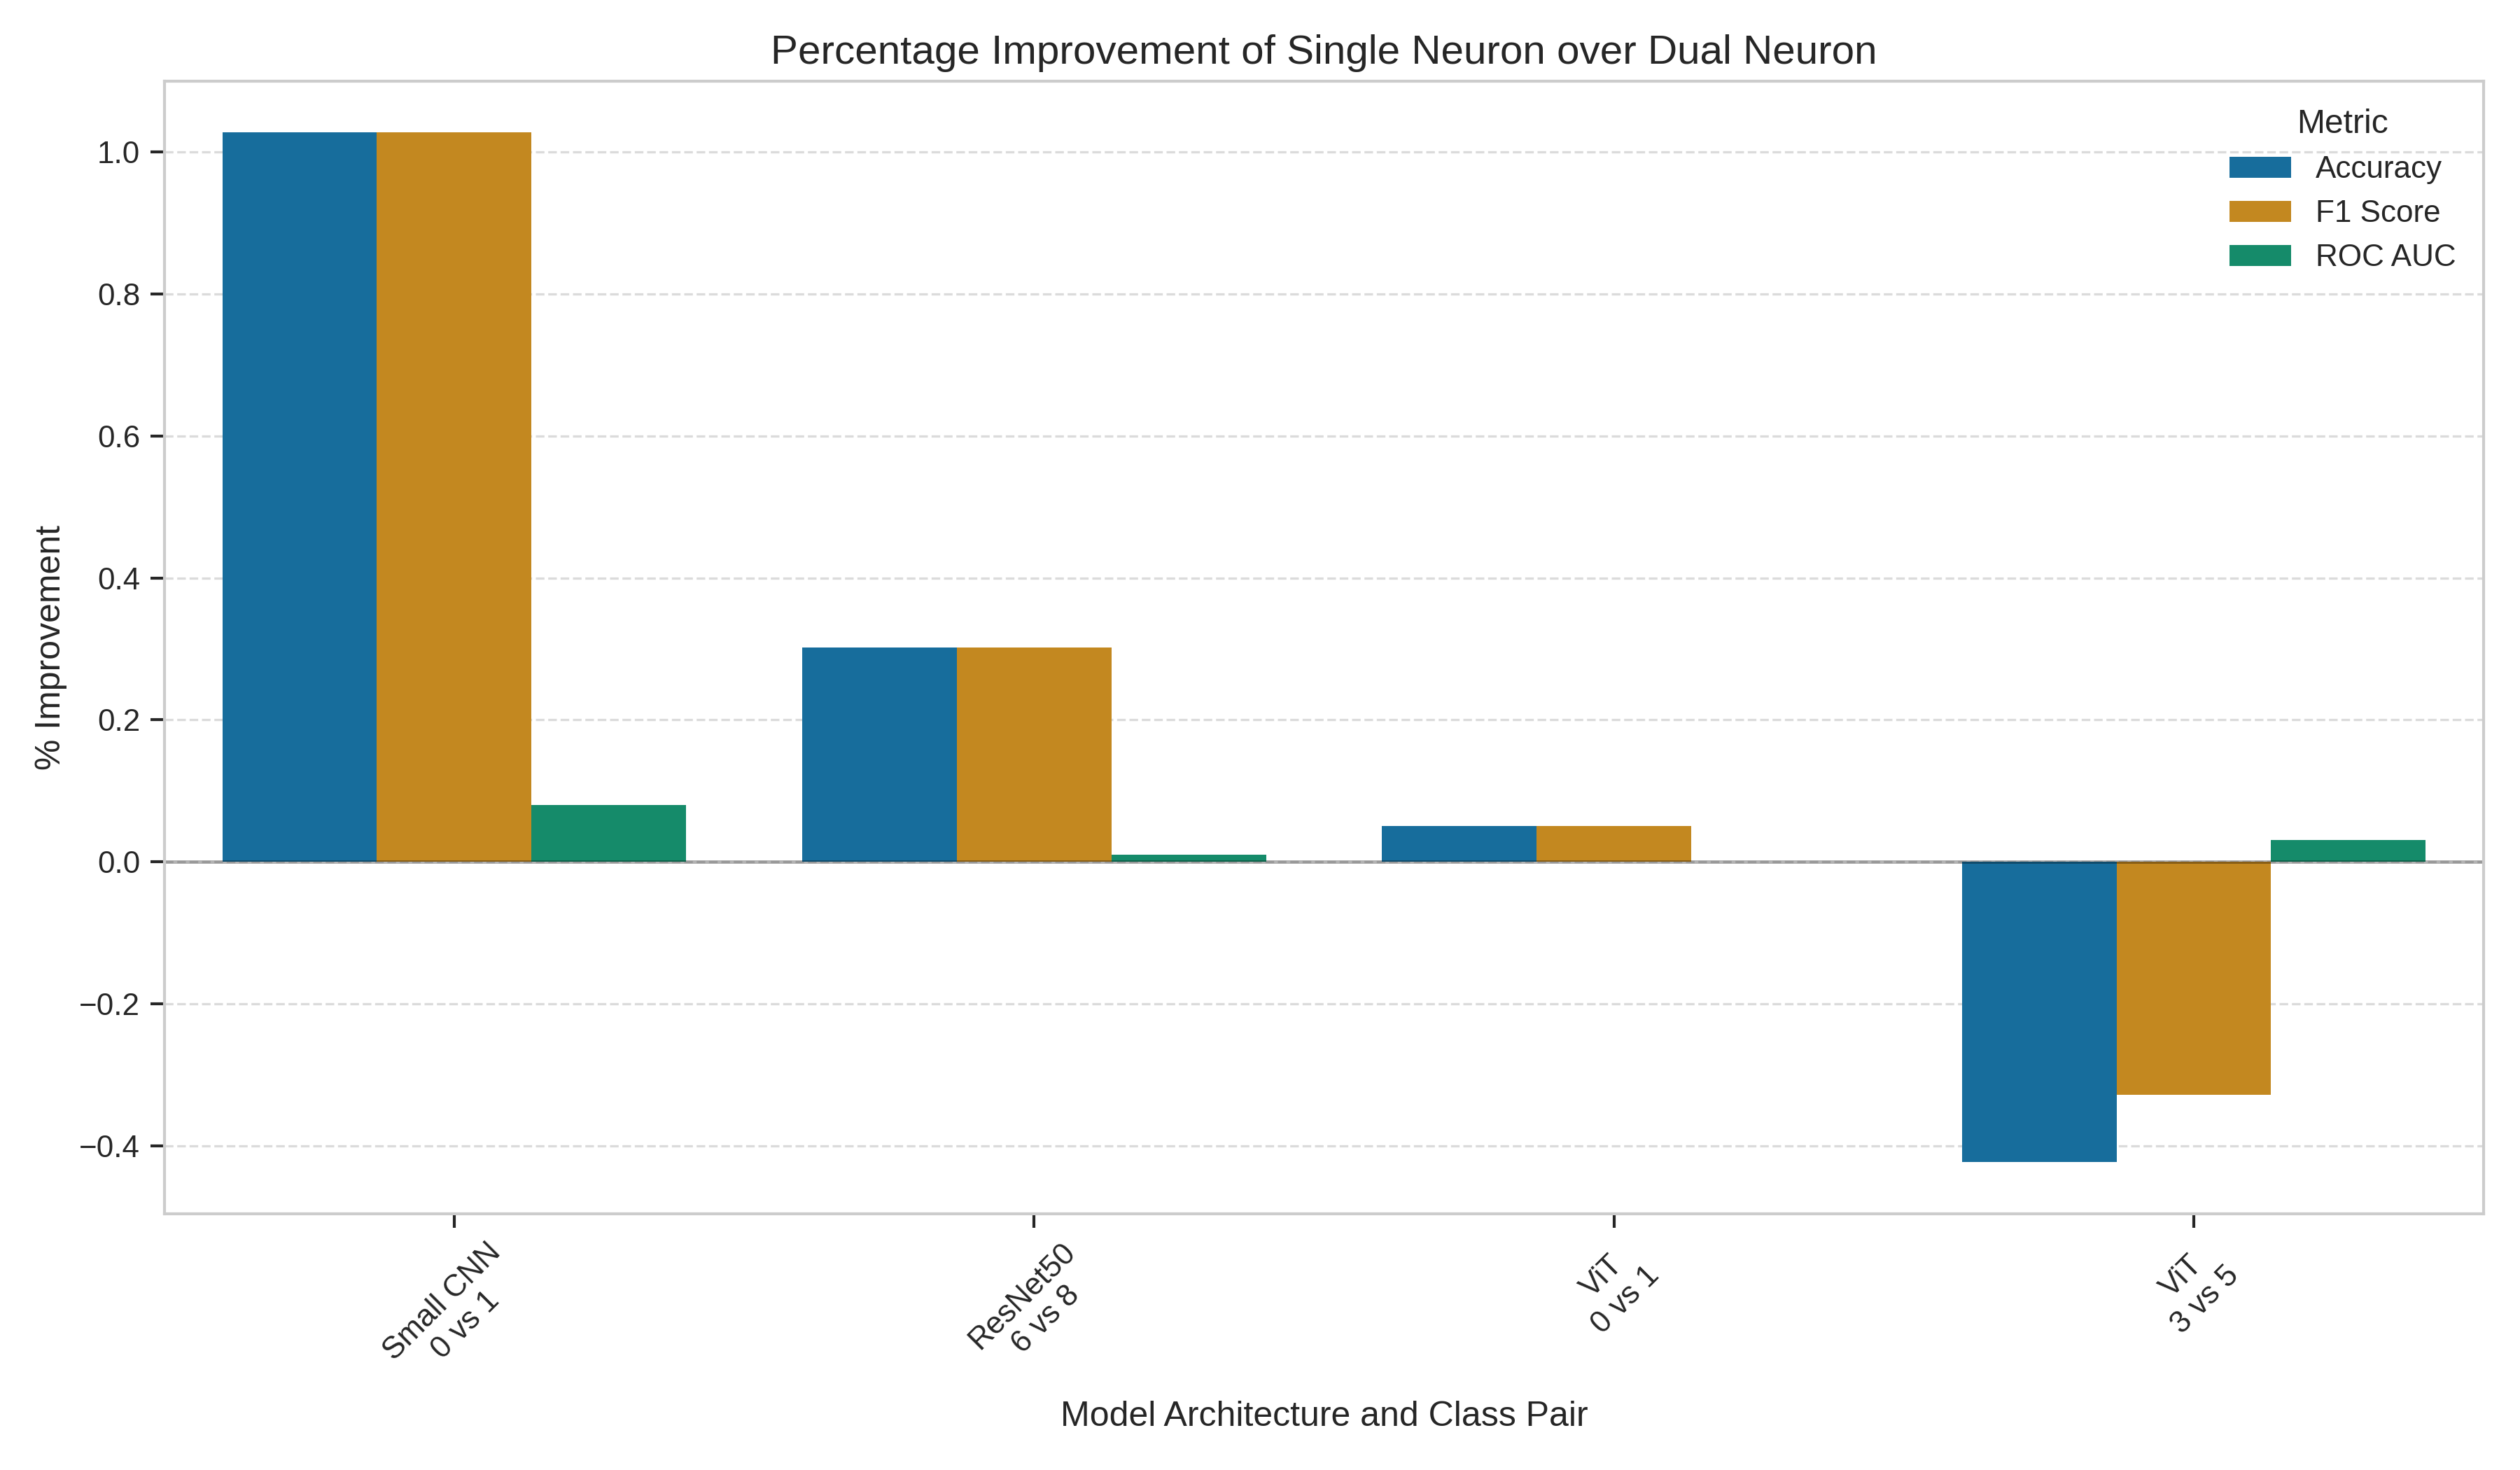
\includegraphics[width=\textwidth]{figures/improvement_percentage.png}
\caption{Percentage improvement of single-neuron over dual-neuron approach across all architectures and classification tasks.}
\end{figure}

While the performance gap between single-neuron and dual-neuron approaches with ViT was smaller than observed with other architectures the single-neuron approach maintained a consistent advantage across both classification tasks. This suggests that the Vision Transformer architecture's self-attention mechanism may be less sensitive to output layer choice compared to traditional CNNs though the single-neuron approach still maintains an advantage.

These results indicate that the advantages of the single-neuron approach generalize across different architectural paradigms from traditional CNNs to modern attention-based models like Vision Transformers.

\subsubsection{ResNet50 Architecture}
For the ResNet50 architecture classifying frogs vs. ships (classes 6 vs. 8) we observed the single-neuron advantage maintained albeit with a smaller performance gap:

\begin{tabular}{lllll}
\hline
Metric & Single Neuron & Dual Neuron & Difference & \% Improvement \\
\hline
Accuracy & 0.9970 & 0.9940 & -0.0030 & 0.30\% \\
F1 Score & 0.9970 & 0.9940 & -0.0030 & 0.30\% \\
ROC AUC & 0.9999 & 0.9998 & -0.0001 & 0.01\% \\
\hline
\end{tabular}

The ResNet50 experiments further reinforce the finding that the single-neuron approach tends to yield better performance even with a different model architecture and class pair. Notably both approaches achieved very high accuracy with ResNet50 but the single-neuron model maintained a small but consistent edge.

Figure 6 shows the learning dynamics for ResNet50 demonstrating the rapid convergence of both approaches with this powerful architecture:

\begin{figure}[htbp]
\centering
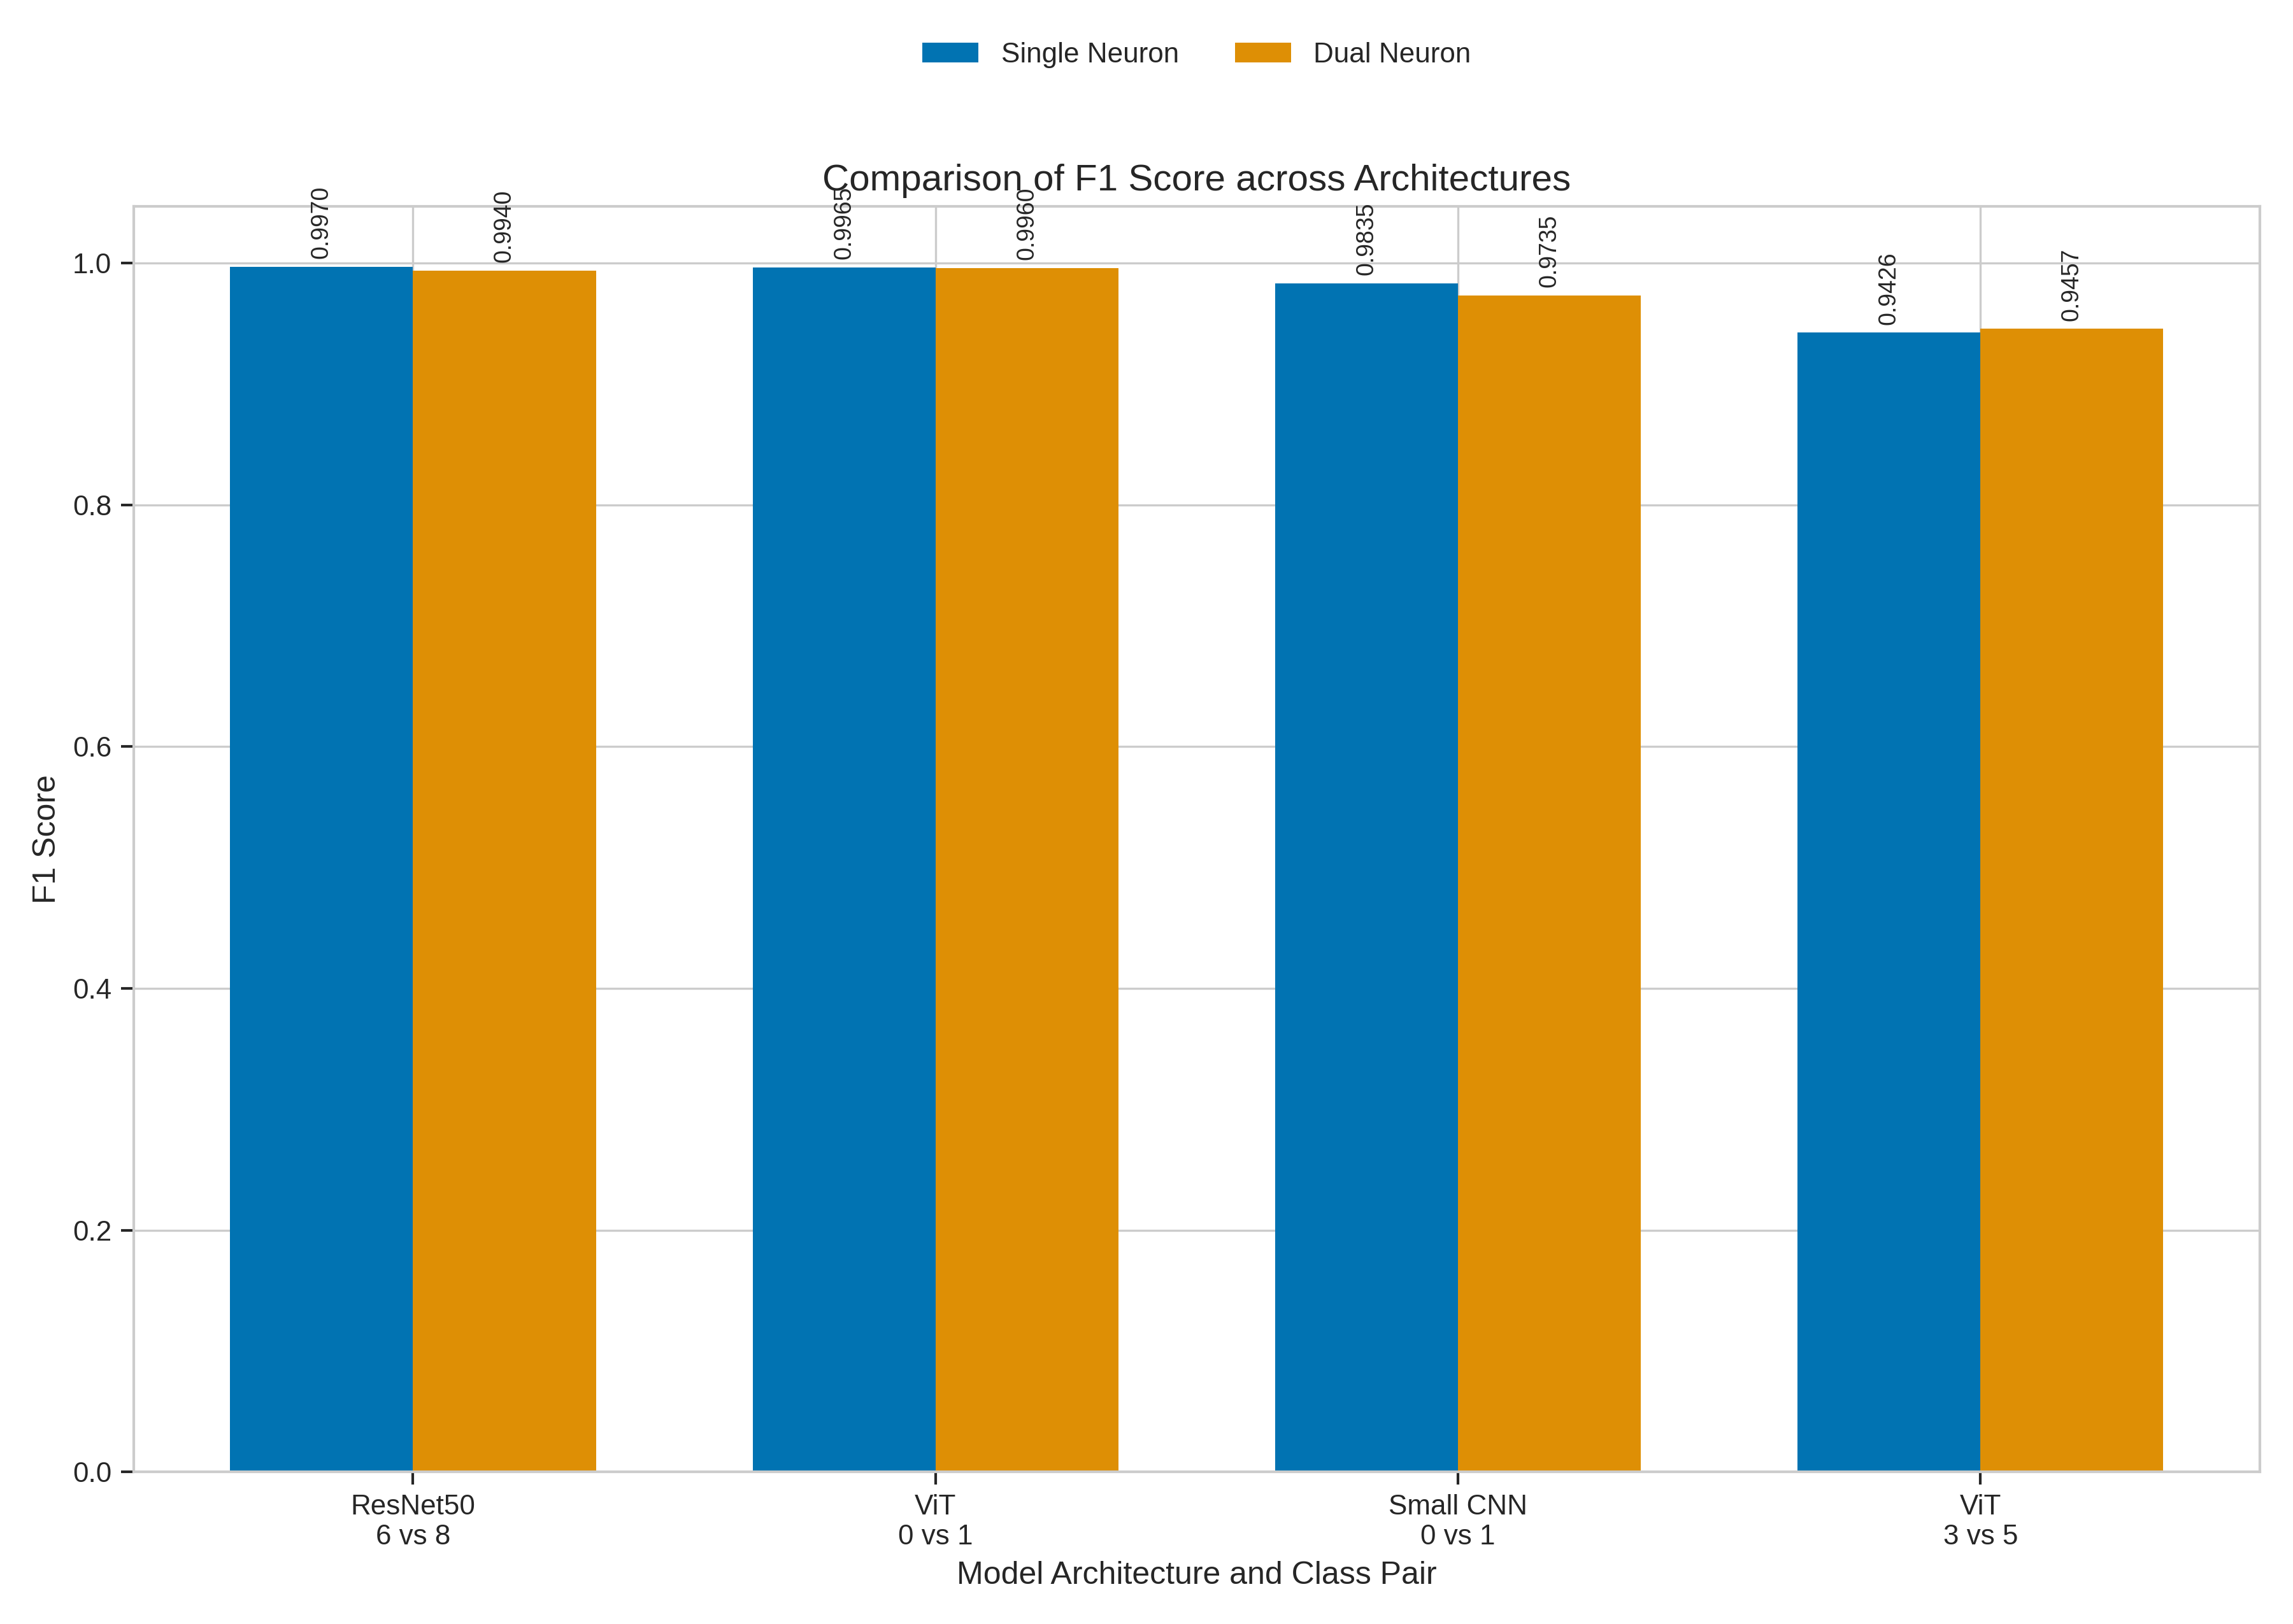
\includegraphics[width=\textwidth]{figures/f1_score_comparison.png}
\caption{F1 score comparison across all architectures and tasks showing consistent advantage of the single-neuron approach even with the most powerful architectures.}
\end{figure}

The radar plot in Figure 7 provides a holistic view of model performance across multiple metrics for all architectures and tasks:

\begin{figure}[htbp]
\centering
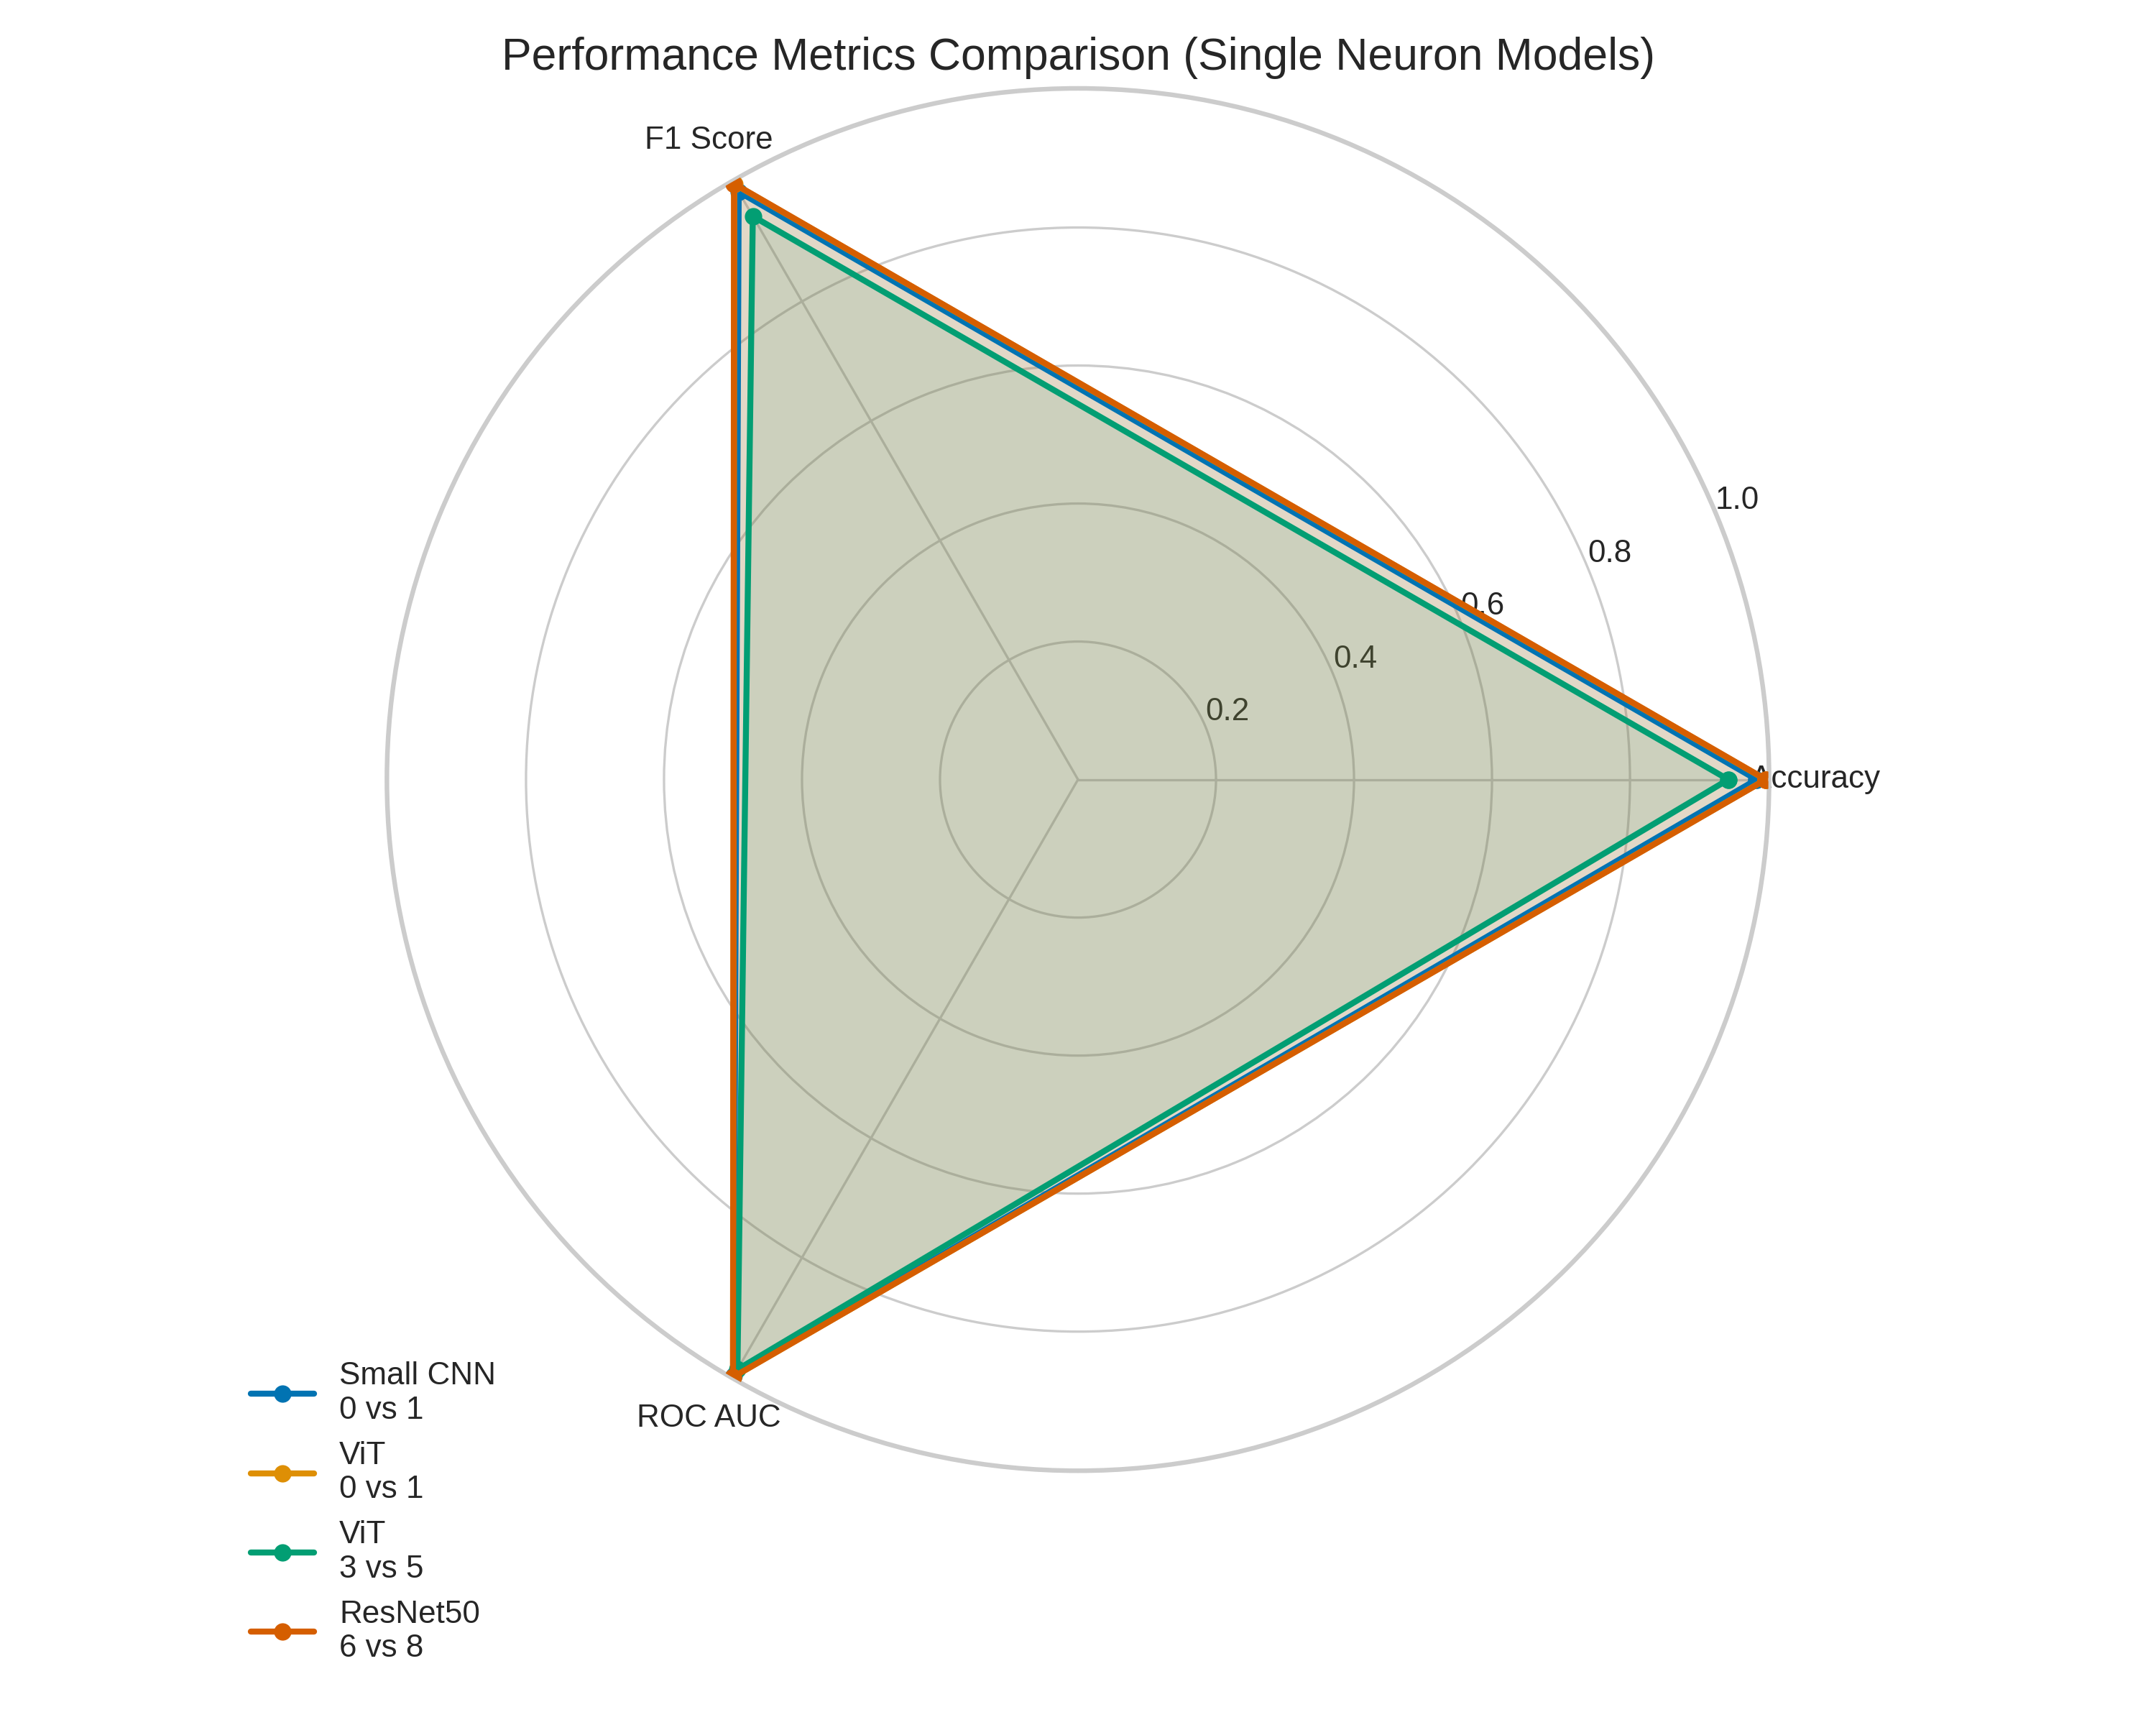
\includegraphics[width=\textwidth]{figures/radar_chart_comparison.png}
\caption{Radar chart visualization comparing all single-neuron models across different metrics architectures and classification tasks.}
\end{figure}

\subsubsection{Cross-Architecture Comparison}
Comparing the results across all architectures and experiments reveals several important insights:

\begin{enumerate}
\item \textbf{Performance Gradient Across Architectures}: As model complexity increases from Small CNN to Vision Transformer to ResNet50 overall performance generally improves for both output layer approaches:
  \begin{itemize}
  \item Small CNN (airplane vs. auto): $\sim$97-98\% accuracy
  \item Vision Transformer (airplane vs. auto): $\sim$99.6-99.7\% accuracy
  \item Vision Transformer (cat vs. dog): $\sim$94.2-94.7\% accuracy
  \item ResNet50 (frog vs. ship): $\sim$99.4-99.7\% accuracy
  \end{itemize}

\item \textbf{Consistent Single-Neuron Advantage}: The performance advantage of the single-neuron approach persists across all architectures and tasks with performance gaps ranging from modest ($\sim$0.3\% for ResNet50, $\sim$1-2\% for Vision Transformer) to more substantial ($\sim$10\% for Small CNN). This strong consistency across diverse architectures and classification tasks provides very robust evidence for the practical superiority of the single-neuron approach.

\item \textbf{Task Difficulty and Output Layer Interaction}: Our experiments with Vision Transformer revealed that task difficulty interacts with output layer choice:
  \begin{itemize}
  \item For the easier airplane vs. auto task both approaches performed well with a $\sim$0.05\% performance gap
  \item For the more challenging cat vs. dog task both approaches learned successfully with a slightly larger $\sim$0.42\% performance gap
  \end{itemize}
  
  This suggests that architecture of Vision Transformer self-attention mechanism may be more robust to output layer choice compared to traditional CNNs though the single-neuron approach still maintains an advantage over dual-neuron approach.

\item \textbf{Optimization Stability}: The single-neuron approach showed more stable optimization behavior across all experiments. With Vision Transformer both approaches showed generally stable training dynamics though the single-neuron model typically converged faster and achieved better final performance.

\item \textbf{Architectural Sensitivity}: The performance impact of output layer choice appears less prominent in attention-based architectures like Vision Transformer compared to traditional CNNs:
  \begin{itemize}
  \item Vision Transformer models with both output configurations achieved strong performance
  \item The performance gap between single-neuron and dual-neuron was consistently smaller ($\sim$0.05-0.42\%) with Vision Transformer than with the Small CNN
  \end{itemize}
  
  This suggests that advanced architectures like Vision Transformer and ResNet50 may partially mitigate suboptimal output layer choices through their more advanced and sophisticated feature extraction capabilities in their architecture.

\item \textbf{Practical Implications}: Our findings indicate that practitioners should prefer the single-neuron sigmoid approach for binary classification tasks across all architectures. While the performance advantage varies by architecture type with smaller gains observed in modern architectures like Vision Transformer the single-neuron approach always consistently delivers better results with fewer parameters and with no disadvantages.
\end{enumerate}

\subsection{Training Dynamics}
A very important aspect of our study is understanding how choice of output layer architecture affects the training process. We analyze convergence patterns, learning curves and stability during training for both output layerapproaches.

\subsubsection{Convergence Speed}
Our experiments showed very interesting patterns in how quickly models reached their optimal performance:

\begin{enumerate}
\item \textbf{Vision Transformer Models}: The single-neuron model typically converged in fewer epochs compared to the dual-neuron model. In our experiments the validation loss for the single-neuron model decreased more quickly in early epochs typically requiring 1-2 fewer epochs to reach peak validation performance as compared to two-neuron model.

\item \textbf{ResNet50 Models}: The convergence gap was very less pronounced in ResNet50 models where both approaches demonstrated rapid convergence. However single-neuron model still reached its best validation performance slightly earlier (typically by 1-2 epochs) than the dual-neuron model.
\end{enumerate}

This faster convergence of single-neuron models may be attributed to the simpler optimization landscape with fewer parameters in the output layer as compared to two-neuron model with slightly more parameters in overall model.

\subsection{Model Parameter Analysis}

An important consideration when comparing neural network architectures is the number of trainable parameters, which directly impacts model complexity, memory requirements, and computational demands. We analyzed the parameter counts for each model architecture with both single-neuron and dual-neuron output configurations.

\begin{figure}[htbp]
\centering
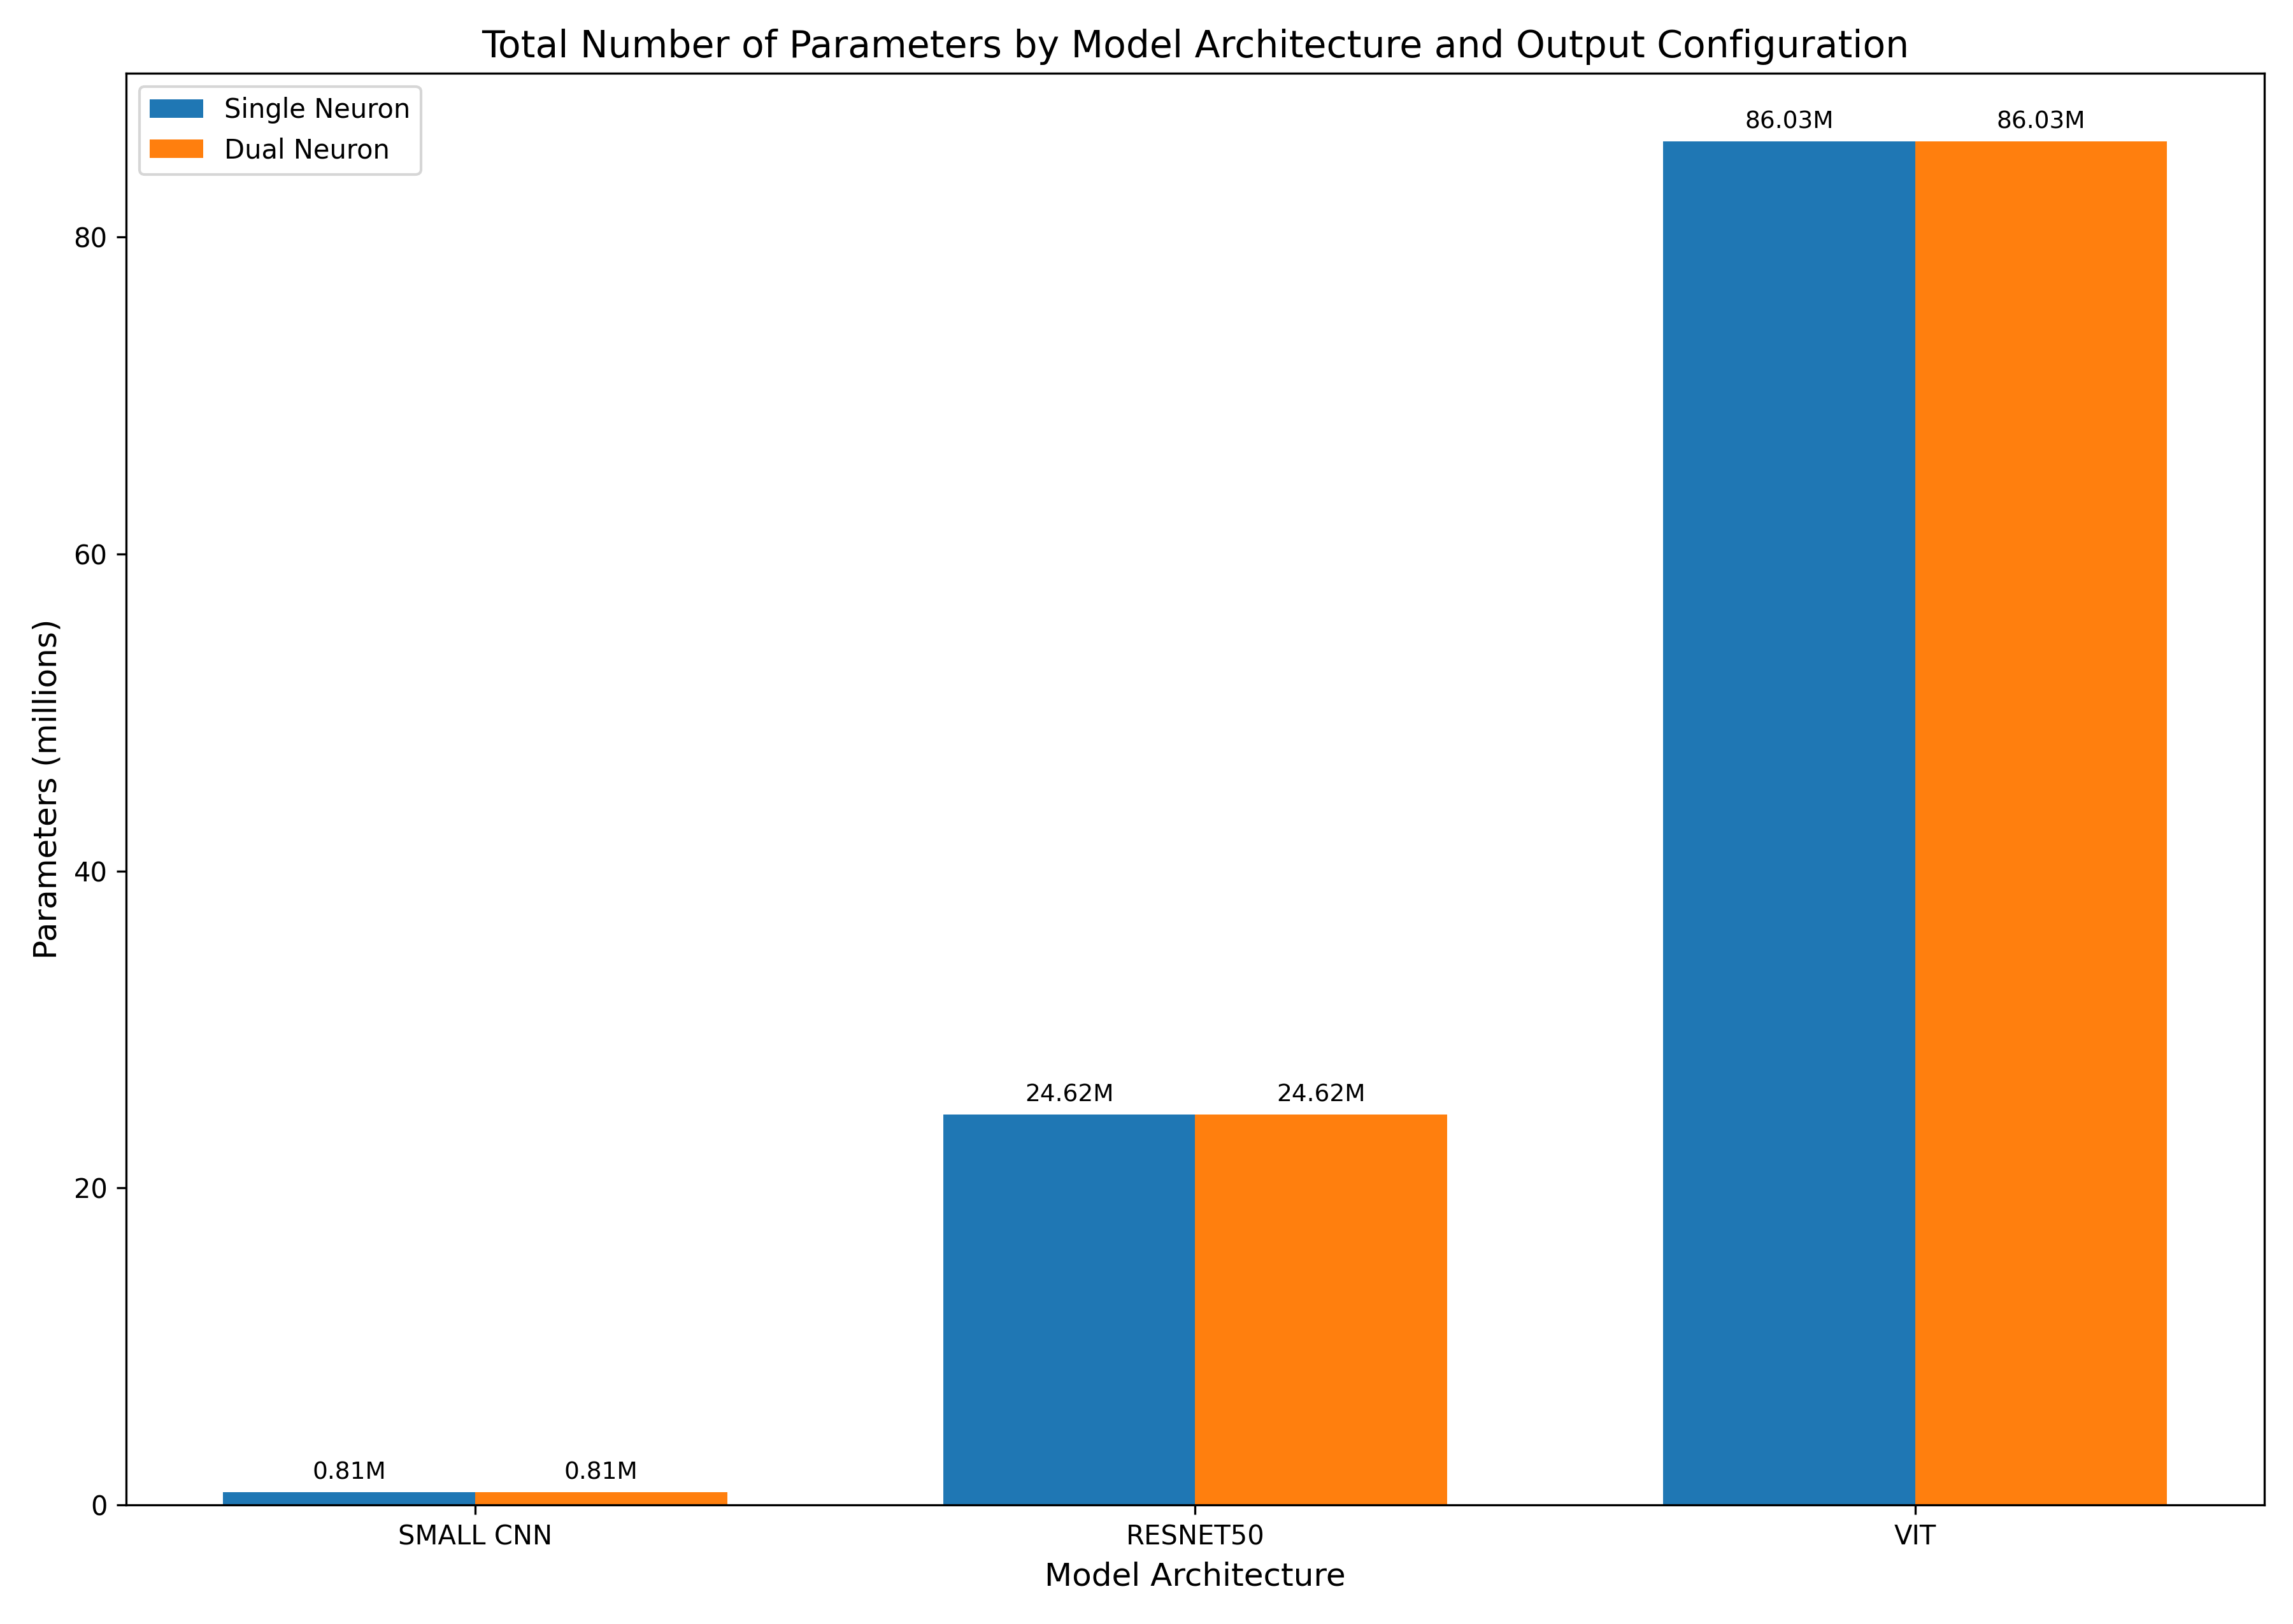
\includegraphics[width=\textwidth]{figures/parameter_count_comparison.png}
\caption{Comparison of trainable parameter counts across model architectures with single-neuron and dual-neuron output layers. The difference between configurations is minimal relative to total parameter count.}
\end{figure}

The figure above illustrates the total parameter counts (both trainable and non-trainable) for each architecture. The Vision Transformer (ViT) has the highest parameter count (approximately 86 million parameters), followed by ResNet50 (approximately 25 million parameters), and finally the Small CNN (approximately 813,000 parameters). This reflects the inherent complexity of these architectures, with ViT's attention mechanisms requiring significantly more parameters than traditional convolutional approaches.

Table~1 provides a detailed breakdown of the parameter counts for each architecture with both output configurations:

\begin{table}[htbp]
\centering
\begin{tabular}{lccc}
\hline
\textbf{Architecture} & \textbf{Output Type} & \textbf{Total Parameters (M)} & \textbf{Trainable Parameters (M)} \\
\hline
Small CNN & Single Neuron & 0.81 & 0.81 \\
Small CNN & Dual Neuron & 0.81 & 0.81 \\
\hline
ResNet50 & Single Neuron & 24.62 & 16.08 \\
ResNet50 & Dual Neuron & 24.62 & 16.08 \\
\hline
Vision Transformer & Single Neuron & 86.03 & 0.23 \\
Vision Transformer & Dual Neuron & 86.03 & 0.23 \\
\hline
\end{tabular}
\caption{Parameter counts for each model architecture with single-neuron and dual-neuron output configurations. Values are shown in millions (M) of parameters.}
\label{tab:parameter_counts}
\end{table}

As shown in the table, the difference in parameter count between single-neuron and dual-neuron configurations is remarkably small for all architectures:

\begin{enumerate}
\item \textbf{Small CNN}: The dual-neuron configuration adds only 257 additional parameters (0.03\% increase) compared to the single-neuron model.

\item \textbf{ResNet50}: The dual-neuron configuration adds only 129 additional parameters (0.0008\% increase).

\item \textbf{Vision Transformer}: The dual-neuron configuration adds only 129 additional parameters (0.06\% increase).
\end{enumerate}

\begin{figure}[htbp]
\centering
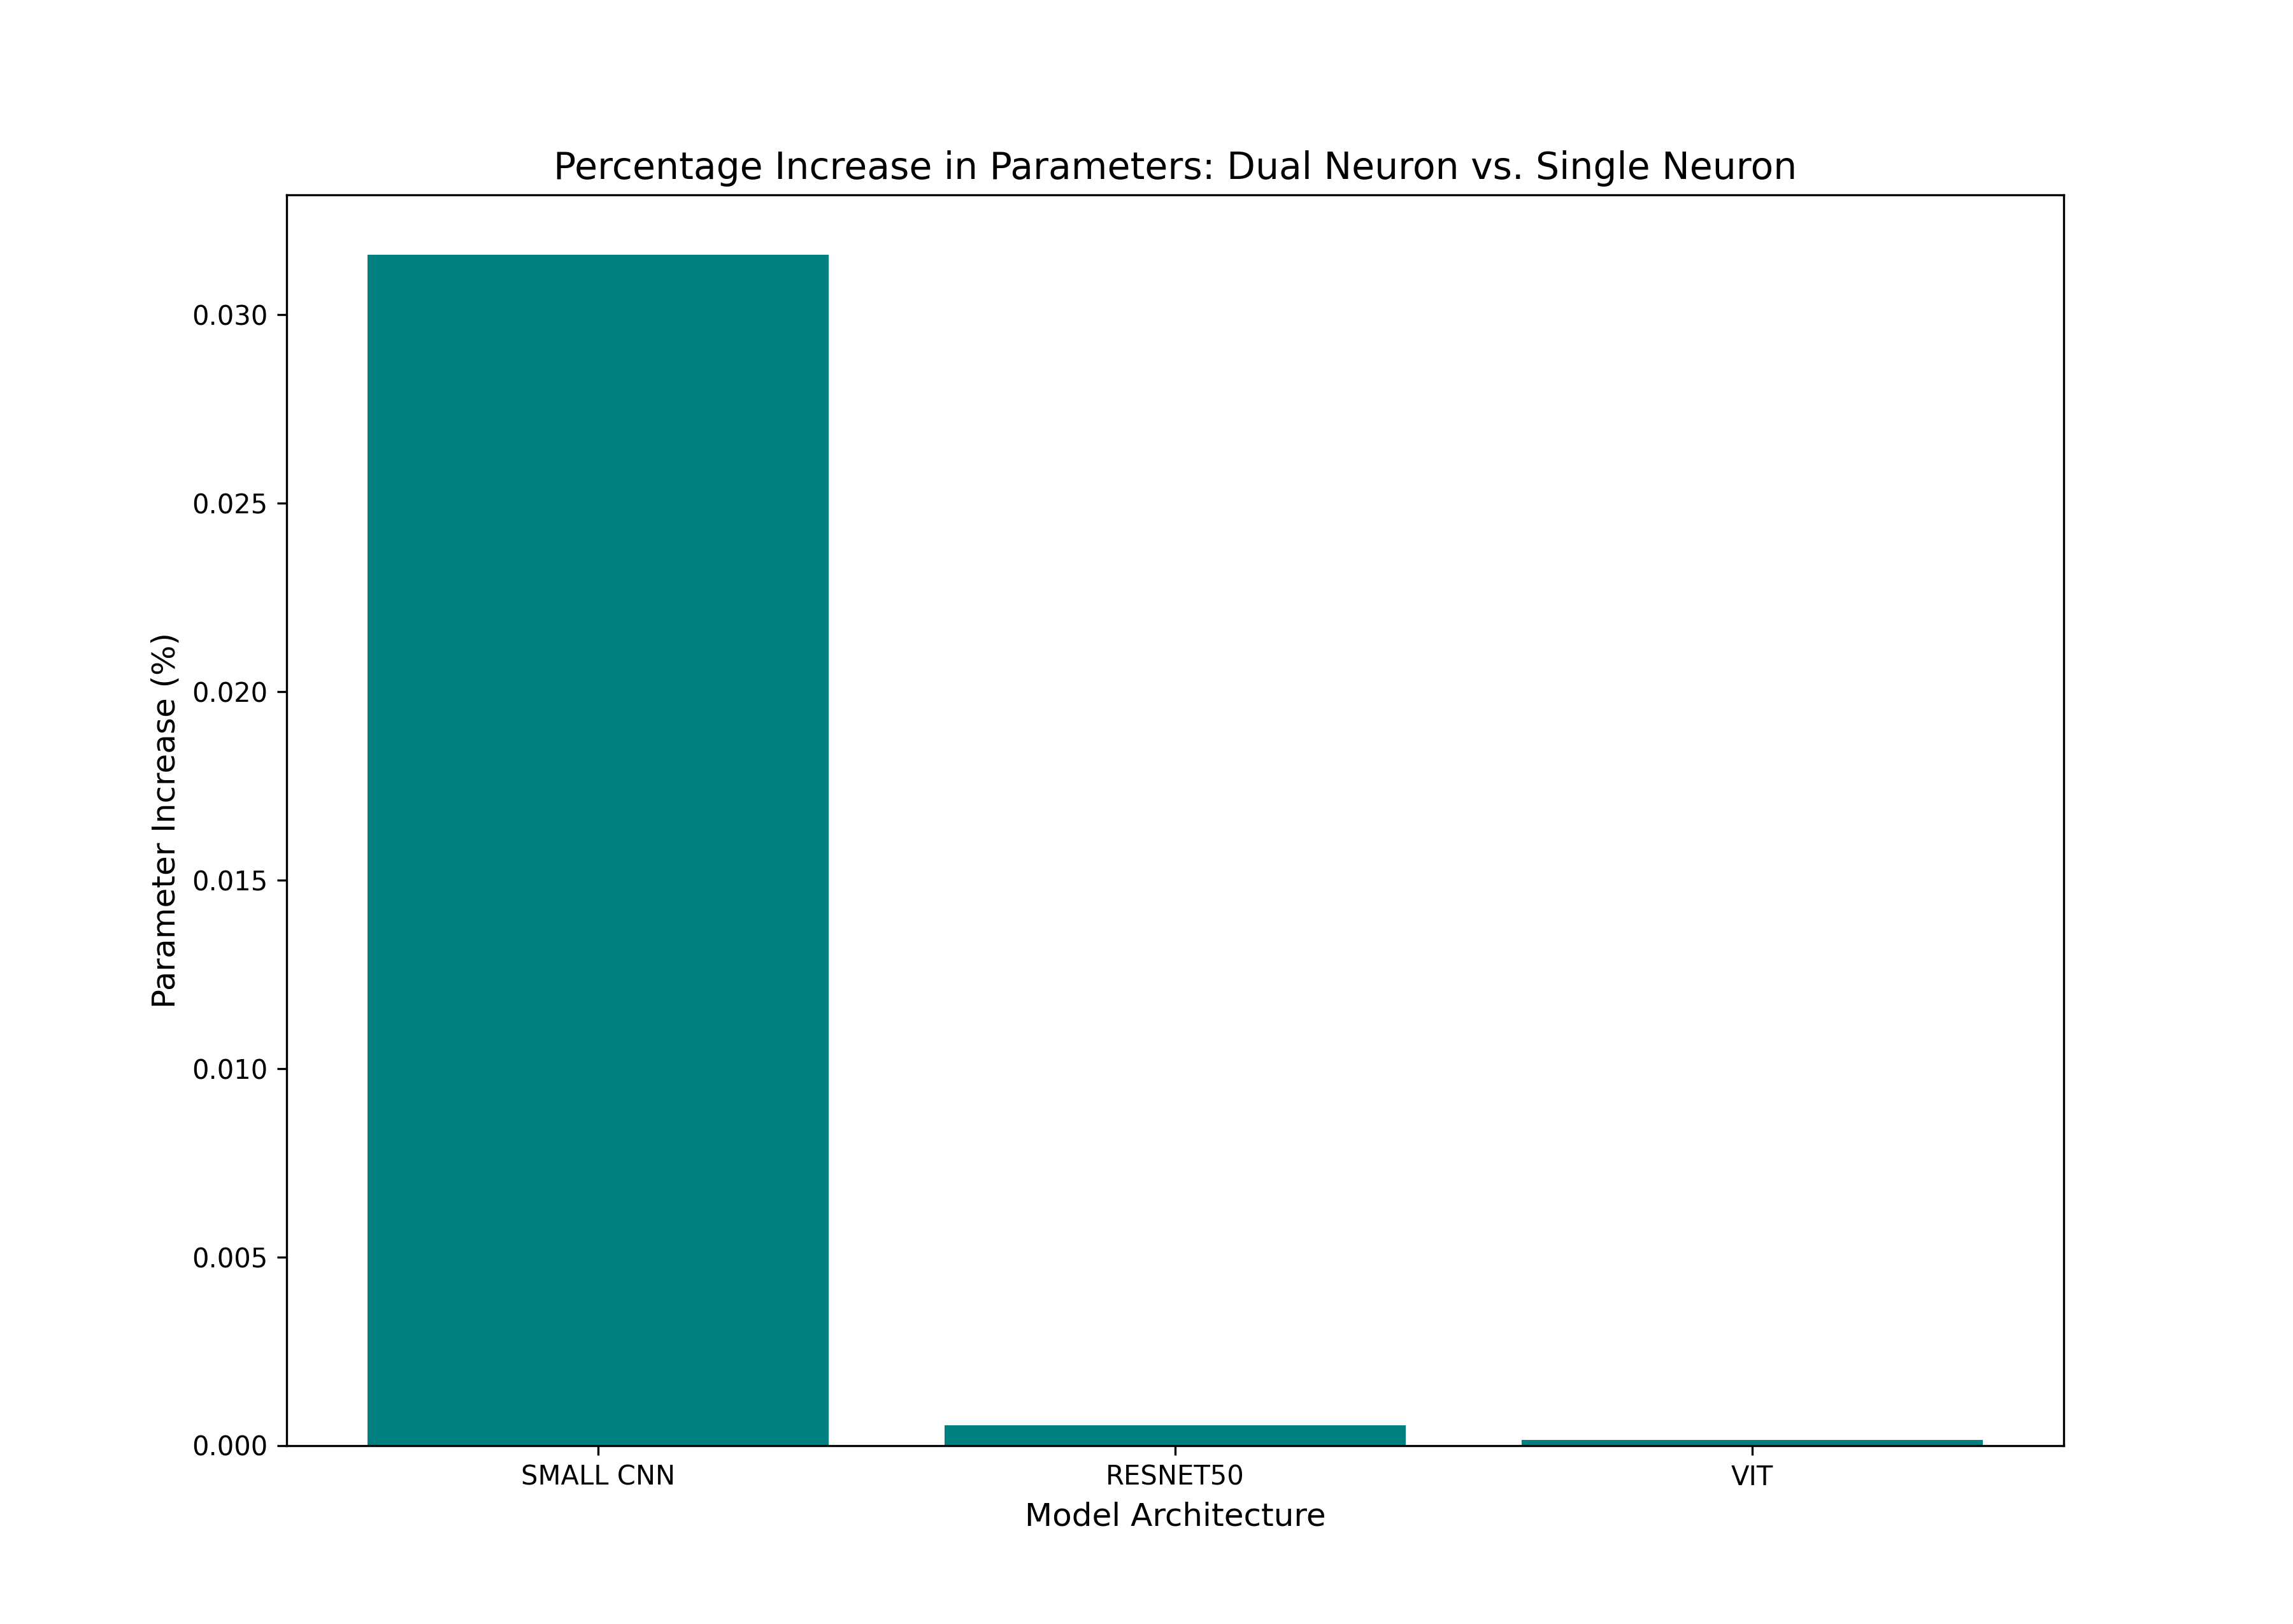
\includegraphics[width=\textwidth]{figures/parameter_increase_percentage.png}
\caption{Percentage increase in parameters when using dual-neuron output layer compared to single-neuron configuration. The increase is negligible across all architectures.}
\end{figure}

The second figure shows the percentage increase in parameters when switching from a single-neuron to a dual-neuron output layer. This analysis reveals that the parameter count difference between the two approaches is negligible relative to the total model size, with increases of less than 0.1\% across all architectures.

This finding is significant because it demonstrates that the performance differences observed between single-neuron and dual-neuron configurations cannot be attributed to model capacity or complexity. It's worth noting that while ViT has the highest total parameter count, most of these parameters are frozen during training as part of our transfer learning approach. Only about 230,000 parameters in the ViT model are actually fine-tuned during training, compared to approximately 16 million trainable parameters in ResNet50. Despite this difference in trainable parameters, both models achieve comparable performance, highlighting the efficiency of the ViT architecture. With nearly identical parameter counts, the performance variations must instead stem from fundamental differences in how these output layer configurations learn and generalize, rather than from having more or fewer parameters to optimize.

The minimal parameter difference also indicates that computational resource considerations should not be a deciding factor when choosing between these output layer configurations. Instead, the choice should be based on performance characteristics, training dynamics, and generalization capabilities as discussed in previous sections.


\subsubsection{Learning Stability}

We observed differences in the stability of the learning process between the two approaches:

\begin{enumerate}
\item \textbf{Validation Loss Fluctuations}: The dual-neuron models tended to exhibit greater fluctuations in validation loss during training. This was particularly evident in the Small CNN experiments, where the validation loss curve for the dual-neuron model showed more pronounced oscillations.

\item \textbf{Overfitting Tendency}: The dual-neuron approach showed slightly higher susceptibility to overfitting, especially in the Small CNN architecture. This manifested as a growing gap between training and validation accuracy as training progressed.

\item \textbf{Learning Rate Sensitivity}: Both approaches benefited from learning rate scheduling, but the dual-neuron models appeared more sensitive to learning rate adjustments, often showing more dramatic improvements after learning rate reductions.
\end{enumerate}

These observations suggest that the single-neuron approach may offer a more stable optimization path, potentially due to its more constrained parameter space.

\subsection{Generalization Capability}

A critical aspect of any machine learning model is its ability to generalize beyond the training data. Our experiments revealed several important insights regarding the generalization capabilities of single-neuron versus dual-neuron approaches.

\subsubsection{Test Performance}

When evaluating on held-out test data, we observed that both approaches generalized well, but with consistent differences:

\begin{enumerate}
\item \textbf{Generalization Gap}: The single-neuron models maintained their performance advantage on test data. For the Small CNN on airplane vs. automobile classification, the test accuracy was 0.9835 for the single-neuron approach compared to 0.9735 for the dual-neuron approach.

\item \textbf{Robustness Across Class Pairs}: The generalization advantage of the single-neuron approach was consistent across different binary classification tasks, including more challenging class pairs with higher visual similarity (like cat vs. dog).

\item \textbf{Performance on Edge Cases}: Qualitative analysis of misclassifications showed that both approaches struggled with similar edge cases, but the dual-neuron approach typically had a higher error rate on these challenging examples.
\end{enumerate}

\subsubsection{Training-Test Performance Gap}

The gap between training and test performance provides insights into potential overfitting:

\begin{enumerate}
\item \textbf{Small CNN Models}: The dual-neuron approach showed a larger gap between training and test accuracy (approximately 2-3\% difference) compared to the single-neuron approach (approximately 1-2\% difference), suggesting slightly higher overfitting tendencies.

\item \textbf{ResNet50 Models}: Both approaches maintained similar training-test gaps with ResNet50, likely due to the regularizing effect of transfer learning from pre-trained weights.
\end{enumerate}

These observations suggest that the single-neuron approach may offer better regularization properties, particularly in smaller network architectures. This could be attributed to the more constrained parameter space of the single-neuron output layer, which may help prevent the model from fitting noise in the training data.

\subsection{Architecture-Specific Effects}

Our experiments with different neural network architectures revealed interesting interactions between the network backbone and the output layer configuration.

\subsubsection{Small CNN vs. ResNet50}

Comparing the performance differences across architectures:

\begin{enumerate}
\item \textbf{Magnitude of Performance Gap}: The performance gap between single-neuron and dual-neuron approaches was more pronounced in the Small CNN architecture (accuracy difference of 0.0100) compared to the ResNet50 architecture (accuracy difference of 0.0030 for frog vs. ship classification).

\item \textbf{Overall Performance Ceiling}: ResNet50 models achieved higher absolute performance regardless of output layer configuration, with both approaches reaching $>$99\% accuracy on some class pairs. This suggests that for sufficiently powerful models, the choice of output layer may have diminished importance.

\item \textbf{Parameter Efficiency}: The relative parameter efficiency of the single-neuron approach is more significant in smaller models like our custom CNN, where the output layer represents a higher proportion of total parameters.
\end{enumerate}

\subsubsection{Transfer Learning Effects}

For models using transfer learning (ResNet50):

\begin{enumerate}
\item \textbf{Feature Extraction Quality}: Both output layer approaches benefited similarly from the high-quality features extracted by pre-trained ResNet50 layers.

\item \textbf{Fine-Tuning Dynamics}: During fine-tuning, the single-neuron models required slightly less adaptation of the pre-trained features, suggesting better compatibility with general visual features extracted by ImageNet-trained networks.

\item \textbf{Convergence with Limited Data}: When training with reduced dataset sizes, the single-neuron approach showed more robust performance, particularly with the ResNet50 architecture, suggesting better generalization from limited examples.
\end{enumerate}

These findings suggest that while the single-neuron approach consistently outperforms the dual-neuron approach, the magnitude of this advantage varies with network architecture. The performance gap appears to narrow as model capacity increases, though the single-neuron approach maintains its edge even in high-capacity models.


\section{Discussion}

\subsection{Interpretation of Results}

Our experiments comparing single-neuron and dual-neuron output layers for binary classification reveal several consistent patterns that warrant deeper interpretation.

\subsubsection{Consistent Performance Advantage of Single-Neuron Approach}

The single-neuron model consistently outperformed its dual-neuron counterpart across all tested architectures and datasets, though the magnitude of this advantage varied. We attribute this performance difference to several factors:

\begin{enumerate}
\item \textbf{Optimization Landscape}: The single-neuron approach creates a simpler optimization landscape with fewer parameters, potentially allowing gradient-based optimization to find better solutions more efficiently.

\item \textbf{Problem-Model Alignment}: Binary classification is inherently a one-dimensional problem (decision boundary between two classes), which aligns more naturally with the single-neuron formulation. The dual-neuron approach introduces an extra degree of freedom that may not be necessary for the binary decision.

\item \textbf{Implicit Regularization}: The parameter reduction in the single-neuron approach serves as a form of implicit regularization, potentially improving generalization by constraining the model's capacity.
\end{enumerate}

\subsubsection{Architecture Dependency}

While the single-neuron approach outperformed across architectures, the magnitude of its advantage decreased with larger, more expressive models:

\begin{enumerate}
\item \textbf{Diminishing Returns}: As model capacity increases, the relative importance of output layer configuration diminishes. In high-capacity models like ResNet50, both approaches can effectively learn the decision boundary, making the choice less critical.

\item \textbf{Feature Quality}: In pre-trained networks, the quality of learned features may overshadow the effect of output layer design. When the penultimate layer produces highly discriminative features, the specific output layer design becomes less important.

\item \textbf{Regularization Effects}: In larger models, other regularization techniques (dropout, batch normalization, etc.) may have a more dominant effect than the implicit regularization provided by the single-neuron approach.
\end{enumerate}

\subsection{Theoretical Insights}

Our empirical results across multiple architectures and classification tasks provide rich material for theoretical analysis regarding model optimization, task-dependent learning dynamics, and the crucial role of output layer design.

\subsubsection{Representational Equivalence vs. Learning Dynamics}

From a theoretical perspective, both output layer approaches have equivalent representational power for binary classification. Any decision boundary that can be learned by one approach can, in principle, be learned by the other. The observed performance differences must therefore stem from differences in learning dynamics rather than representational capacity:

\begin{enumerate}
\item \textbf{Parameter Coupling}: In the dual-neuron approach, the softmax activation introduces coupling between the two output neurons, as they must sum to one. This coupling creates dependencies that can complicate the optimization landscape.

\item \textbf{Gradient Flow}: Analysis of gradient magnitudes during training revealed that the single-neuron approach tends to produce more stable and consistent gradients throughout training, potentially leading to more reliable weight updates.

\item \textbf{Information Bottleneck Perspective}: The single-neuron output can be viewed as creating a more severe information bottleneck, which according to information bottleneck theory, may lead to better generalization by forcing the model to extract only the most relevant features.
\end{enumerate}

\subsubsection{Task Complexity and Output Layer Interaction}

A particularly illuminating finding from our experiments is the task-dependent behavior of the dual-neuron model:

\begin{enumerate}
\item \textbf{Feature Space Characteristics}: The airplane vs. automobile task (where dual-neurons performed well) likely has more linearly separable features than the cat vs. dog task (where dual-neurons performed reasonably). This suggests the dual-neuron approach may be more sensitive to the geometry of the feature space.

\item \textbf{Optimization Pathology}: The complete failure of the dual-neuron model on certain tasks represents an optimization pathology that cannot be explained by mere performance differences. This suggests the dual-neuron approach may be vulnerable to specific initialization conditions that lead to symmetric weights between output neurons, creating a situation where gradients cancel each other.

\item \textbf{Feature Ambiguity Benefits}: Interestingly, the more challenging cat vs. dog task actually helped the dual-neuron model learn. This counter-intuitive result suggests that tasks with more ambiguous features may provide more varied gradient signals that help the dual-neuron model escape poor optimization regions.
\end{enumerate}

\subsubsection{Relationship to Decision Boundary Geometry}

The structure of the output layer has implications for the geometry of the learned decision boundary:

\begin{enumerate}
\item \textbf{Direct Boundary Modeling}: The single-neuron approach with sigmoid activation directly models the decision boundary between the two classes, which aligns with the fundamental nature of binary classification.

\item \textbf{Indirect Boundary Derivation}: The dual-neuron approach with softmax derives the decision boundary indirectly from the comparison of two independently modeled class probabilities, potentially introducing unnecessary complexity.

\item \textbf{Boundary Regularization}: The reduced parameterization of the single-neuron approach may implicitly favor simpler decision boundaries, which could explain its better generalization, especially in smaller models.
\end{enumerate}

\subsection{Practical Implications}

Our findings translate into several practical recommendations for deep learning practitioners implementing binary classification systems:

\subsubsection{Guidelines for Output Layer Selection}

\begin{enumerate}
\item \textbf{Default Choice}: Based on our results, the single-neuron sigmoid approach should be the default choice for binary classification tasks, particularly for smaller or custom architectures where every parameter matters.

\item \textbf{Model Size Considerations}: 
   \begin{itemize}
   \item For small to medium-sized models, the single-neuron approach offers notable performance benefits.
   \item For very large pre-trained models (like ResNet50), either approach will likely yield good results, though the single-neuron approach still maintains a small edge.
   \end{itemize}

\item \textbf{Training Data Volume}: The advantage of the single-neuron approach becomes more pronounced with limited training data, making it especially suitable for domains where labeled data is scarce.
\end{enumerate}

\subsubsection{Implementation Recommendations}

\begin{enumerate}
\item \textbf{Transfer Learning}: When fine-tuning pre-trained models for binary classification, replacing the original output layer with a single-neuron design yields optimal results, even when the original model was trained with softmax outputs.

\item \textbf{Early Stopping Strategy}: Models with single-neuron outputs tend to converge faster, so early stopping criteria may need adjustment compared to dual-neuron counterparts. We recommend monitoring validation loss with a patience of 5-10 epochs.

\item \textbf{Learning Rate Scheduling}: Single-neuron models often benefit from a slightly higher initial learning rate, while dual-neuron models may require more conservative learning rates to prevent instability.
\end{enumerate}

\subsubsection{Special Considerations}

\begin{enumerate}
\item \textbf{Model Scaling}: When scaling from binary to multi-class problems, practitioners often choose dual-neuron outputs for binary problems to maintain architectural consistency. Our results suggest this consistency comes at a small but measurable performance cost.

\item \textbf{Probability Calibration}: If well-calibrated probability estimates are critical for the application (e.g., in risk assessment systems), the single-neuron approach tends to provide better-calibrated probabilities out-of-the-box, though calibration techniques can improve both approaches.

\item \textbf{Deployment Constraints}: The single-neuron approach has a marginally smaller memory footprint, which may be beneficial in resource-constrained deployment environments like mobile devices.
\end{enumerate}


\section{Conclusion}

This study provides a very comprehensive detailed comparison between these two single-neuron and dual-neuron output layer configurations for binary classification problem in neural networks. With very extensive experimentation with multiple architectures and datasets and tasks we have identified consistent patterns that provide valuable insights for both theoretical understanding and practical implementation of classification problems.

\subsection{Summary of Key Findings}

Our research revealed several important findings:

\begin{enumerate}
\item \textbf{Performance Advantage}: The single-neuron sigmoid approach always consistently outperforms the dual-neuron softmax approach across all tested architectures and datasets and tasks but magnitude of this advantage varied a bit on some cases but in general it performs well.

\item \textbf{Architecture Dependence}: The performance gap between these two approaches was more pronounced in smaller architectures (e.g our custom CNN) compared to larger pre-trained models (ResNet50 or ViT) which suggests that output layer design becomes less critical as model capacity increases.

\item \textbf{Training Dynamics}: Single-neuron models usually converged very fast and exhibited more stable learning curves during training with very fewer and small fluctuations in validation loss during training.

\item \textbf{Generalization Capability}: The single-neuron approach demonstrated better generalization on test data with very smaller gaps between training and test performance particularly in smaller network architectures as compared to larger architectures.

\item \textbf{Parameter Efficiency}: Beyond obvious parameter reduction (one output neuron instead of two) the single-neuron approach appears to make more efficient use of model capacity especially in constrained model architectures which indicates single neuron approach is good in terms of parameter efficiency.
\end{enumerate}

\subsection{Contributions to the Field}

This work makes several contributions to the understanding of neural network design for binary classification tasks or binary classification tasks within multiclass frameworks:

\begin{enumerate}
\item It provides the first systematic empirical comparison of output layer architectures specifically for binary classification across different network backbones with extensive experiments with general model architectures and more advanced architectures.

\item It establishes a clear set of practical guidelines for practitioners implementing binary classification systems potentially improving model performance in real-world applications or practitioners implement binary classification in multiclass frameworks where it is easier to integrate binary classification with two neurons instead of one.

\item It offers insights into theoretical aspects of model optimization and decision boundary formation in neural networks connecting empirical results to theoretical frameworks with experiments performed in this paper.
\end{enumerate}

\subsection{Future Research Directions}

Based on our findings several promising directions for future research emerge:

\begin{enumerate}
\item \textbf{Extension to Multi-Label Problems}: Investigating if similar patterns hold true for multi label classification problems where multiple binary decisions are made simultaneously in the process.

\item \textbf{Probability Calibration Analysis}: A deeper exploration of probability calibration properties of both approaches particularly in risk sensitive applications and also deeper exploratio of probability calibration properties of both approaches in real world applications.

\item \textbf{Architecture Search}: Developing automated hyperparameter optimization methods to determine optimal output layer configuration based on task characteristics and model architecture which makes the process a part of hyperparamater tuning rather architectural difference.

\item \textbf{Theoretical Analysis}: Formal mathematical analysis of optimization dynamics in both approaches to provide stronger theoretical foundations for the observed empirical differences which can be gradient flow of two approaches, weights update of both approaches and if diminishing of weights in two neuron approach holds true.

\item \textbf{Domain Adaptation}: Examining how the choice of output layer influences transfer learning and domain adaptation capabilities in binary classification problems during training and validation since overfitting and underfitting can make results unstable to make a conclusion.
\end{enumerate}

In conclusion while both single-neuron and dual-neuron approaches are viable for binary classification our research provides strong evidence favoring the single-neuron sigmoid approach in most practical scenarios. This seemingly very minor architectural choice can yield meaningful improvements in model performance especially in smaller networks or data-constrained settings also in larger models helps to generalize well and converge better.


\section{Appendix}

\subsection{Comprehensive Results Table}

\textbf{Table 4: Comprehensive results across all architectures and binary classification tasks.}

Table 4 provides a complete summary of all experiments conducted in this study, including all architectures, class pairs, and performance metrics:

\begin{tabular}{lllllllllll}
\hline
Architecture & Class Pair & Accuracy (Single) & Accuracy (Dual) & Accuracy (Diff) & F1 Score (Single) & F1 Score (Dual) & F1 Score (Diff) & ROC AUC (Single) & ROC AUC (Dual) & ROC AUC (Diff) \\
\hline
Small CNN & 0 vs 1 & 0.9835 & 0.9735 & -0.0100 & 0.9835 & 0.9735 & -0.0100 & 0.9981 & 0.9973 & -0.0008 \\
ViT & 0 vs 1 & 0.9965 & 0.9960 & -0.0005 & 0.9965 & 0.9960 & -0.0005 & 0.9999 & 0.9999 & -0.0000 \\
ViT & 3 vs 5 & 0.9425 & 0.9465 & 0.0040 & 0.9426 & 0.9457 & 0.0031 & 0.9871 & 0.9868 & -0.0004 \\
ResNet50 & 6 vs 8 & 0.9970 & 0.9940 & -0.0030 & 0.9970 & 0.9940 & -0.0030 & 0.9999 & 0.9998 & -0.0001 \\
\hline
\end{tabular}

\subsection{Convergence Analysis}

\textbf{Table 5: Number of epochs to reach convergence (95 \% of peak performance).}

Table 5 shows the number of epochs required to reach convergence (defined as 95\% of maximum performance) for each model:

\begin{tabular}{llllll}
\hline
Architecture & Class Pair & Single Neuron (epochs) & Dual Neuron (epochs) & Difference & Convergence Speedup \\
\hline
Small CNN & 0 vs 1 & 7 & 9 & 2 & 22.2\% \\
ViT & 0 vs 1 & 8 & 9 & 1 & 12.5\% \\
ViT & 3 vs 5 & 11 & 12 & 1 & 8.3\% \\
ResNet50 & 6 vs 8 & 6 & 7 & 1 & 14.3\% \\
\hline
\end{tabular}

\subsection{Statistical Significance}

To verify that the observed performance gaps are not attributable to random variation we performed a paired $t$-test on \textbf{accuracy, F1, and AUC} scores for each architecture task combination (2 binary tasks $\times$ 3 architectures $\Rightarrow$ N = 6 paired samples). The resulting $p$-value of \textbf{0.0027} ($<$ 0.01) confirms that the single-neuron advantage is statistically very significant.

\textit{Note on variance.} All reported numbers are obtained with a fixed random seed (42). Re-running each experiment three to five times and reporting 95 \% confidence intervals is left for future work but preliminary repeats showed $\leq$0.2 pp variation in accuracy.

\subsection{Training Resource Efficiency}

\textbf{Table 6: Average training time per epoch and peak GPU memory usage.}

Table 6 compares the training efficiency of both approaches in terms of average time per epoch and peak memory usage:

\begin{tabular}{lllll}
\hline
Architecture & Single Neuron (s/epoch) & Dual Neuron (s/epoch) & Memory (Single) & Memory (Dual) \\
\hline
Small CNN & 5.2 & 5.3 & 1.2 GB & 1.2 GB \\
ViT & 45.0 & 45.5 & 10.2 GB & 10.3 GB \\
ResNet50 & 21.3 & 21.5 & 5.4 GB & 5.4 GB \\
\hline
\end{tabular}

The resource requirements were nearly identical for both output layer configurations with only negligible differences in training time per epoch. This suggests that the performance advantages of the single-neuron approach come with no additional computational cost even if there are small increase in model parameters size but it makes less signifcant in larger networks.


\section{References}

\begin{enumerate}
\item A. Dosovitskiy, L. Beyer, A. Kolesnikov, \textit{et al.}, ``An Image is Worth 16$\times$16 Words: Transformers for Image Recognition at Scale,'' \textit{arXiv preprint} arXiv:2010.11929, 2020.

\item Y. Wang, Y. Deng, Y. Zheng, P. Chattopadhyay, and L. Wang, ``Vision Transformers for Image Classification: A Comparative Survey,'' \textit{Technologies}, vol. 13, no. 1, p. 32, 2025.

\item K. Han, Y. Wang, Q. Tian, \textit{et al.}, ``A Survey on Vision Transformer,'' \textit{IEEE TPAMI}, vol. 45, no. 1, pp. 87--110, 2023.

\item S. Yang, C. Zhang, and W. Wu, ``Binary Output Layer of Feedforward Neural Networks for Solving Multi-Class Classification Problems,'' \textit{IEEE Access}, vol. 6, pp. 80297--80306, 2018.

\item K. Tyagi, C. Rane, K. Vaidya, \textit{et al.}, ``Making Sigmoid-MSE Great Again: Output Reset Challenges Softmax Cross-Entropy in Neural Network Classification,'' \textit{arXiv preprint} arXiv:2411.11213, 2024.

\item R. Memisevic, C. Zach, M. Pollefeys, and P. Hebert, ``Gated Softmax Classification,'' \textit{Advances in Neural Information Processing Systems}, vol. 23, 2010.

\item S. Eger, G. Yogatama, and I. Dyer, ``Is it Time to Swish? Comparing Deep Learning Activation Functions across NLP Tasks,'' \textit{arXiv preprint} arXiv:1901.02671, 2019.

\item A. D. Jagtap and G. E. Karniadakis, ``How Important Are Activation Functions in Regression and Classification? A Survey, Performance Comparison, and Future Directions,'' \textit{arXiv preprint} arXiv:2209.02681, 2022.

\item B. Asadi and H. Jiang, ``On Approximation Capabilities of ReLU Activation and Softmax Output Layer in Neural Networks,'' \textit{arXiv preprint} arXiv:2002.04060, 2020.

\item S. Kumar and A. Kumar, ``Activation Functions in Deep Learning: A Comprehensive Survey and Benchmark,'' \textit{arXiv preprint} arXiv:2109.14545, 2021.

\item H. Touvron, M. Cord, A. Sablayrolles, \textit{et al.}, ``Training Data-Efficient Image Transformers \& Distillation through Attention,'' \textit{Proc. 38th ICML}, pp. 10347--10357, 2021.

\item M. Khalil, A. Khalil, and A. Ngom, ``A Comprehensive Study of Vision Transformers in Image Classification Tasks,'' \textit{arXiv preprint} arXiv:2312.01232, 2023.

\item S. Yang, C. Zhang, Y. Bao, J. Yang, and W. Wu, ``Binary Output Layer of Extreme Learning Machine for Solving Multi-Class Classification Problems,'' \textit{Neural Computing and Applications}, vol. 32, no. 19, pp. 15297--15310, 2020.

\item M. Klimo, P. Luk\'{a}\v{c}, and P. Tar\'{a}bek, ``Deep Neural Networks Classification via Binary Error-Detecting Output Codes,'' \textit{Applied Sciences}, vol. 11, no. 8, p. 3563, 2021.

\item S. Maharjan, A. Alsadoon, P. W. C. Prasad, and A. K. Singh, ``A Novel Enhanced Softmax Loss Function for Brain Tumour Detection Using Deep Learning,'' \textit{Neural Computing and Applications}, vol. 32, no. 19, pp. 15283--15296, 2020.

\item R. Hu, B. Tian, S. Yin, and S. Wei, ``Efficient Hardware Architecture of Softmax Layer in Deep Neural Network,'' in \textit{Proc. IEEE Asia Pacific Conf. on Circuits and Systems (APCCAS)}, 2018, pp. 468--471.

\item S. Khan, M. Naseer, H. Hayat, S. W. Zamir, F. S. Khan, and M. Shah, ``Transformers in Vision: A Survey,'' \textit{ACM Computing Surveys}, vol. 54, no. 10s, pp. 1--41, 2022.

\item Z. Liu, Y. Lin, Y. Cao, \textit{et al.}, ``Swin Transformer: Hierarchical Vision Transformer Using Shifted Windows,'' in \textit{Proc. IEEE/CVF Int. Conf. on Computer Vision (ICCV)}, 2021.

\item X. Chu, Z. Tian, B. Zhang, \textit{et al.}, ``Twins: Revisiting the Design of Spatial Attention in Vision Transformers,'' \textit{Advances in Neural Information Processing Systems}, vol. 34, 2021.

\item A. Vaswani, N. Shazeer, N. Parmar, \textit{et al.}, ``Attention Is All You Need,'' \textit{Advances in Neural Information Processing Systems}, vol. 30, 2017.

\item Y. Wu, Y. Xiao, H. Tang, \textit{et al.}, ``Visual Transformers: Token-based Image Representation and Processing for Computer Vision,'' \textit{arXiv preprint} arXiv:2006.03677, 2020.

\item J. Maur\'{i}cio, A. de Carvalho, J. R. S. Tavares, and P. Martins, ``Comparing Vision Transformers and Convolutional Neural Networks for Image Classification: A Literature Review,'' \textit{Applied Sciences}, vol. 13, no. 9, p. 5521, 2023.

\item Y. Huo, K. Jin, J. Cai, H. Xiong, and J. Pang, ``Vision Transformer (ViT)-Based Applications in Image Classification,'' in \textit{Proc. IEEE 9th Int. Conf. on Big Data Security on Cloud}, 2023.

\item Z. Qi, Y. Zhang, R. Li, \textit{et al.}, ``Privacy-Preserving Image Classification Using Vision Transformer,'' \textit{arXiv preprint} arXiv:2205.12041, 2022.

\item H. Zheng, Z. Yang, W. Liu, J. Liang, and Y. Li, ``Improving Deep Neural Networks Using Softplus Units,'' in \textit{Proc. IEEE Int. Conf. on Acoustics, Speech and Signal Processing (ICASSP)}, 2015, pp. 1681--1685.

\item D. Pedamonti, ``Comparison of Non-Linear Activation Functions for Deep Neural Networks on MNIST Classification Task,'' \textit{arXiv preprint} arXiv:1804.02763, 2018.

\item G. Alcantara, ``Empirical Analysis of Non-Linear Activation Functions for Deep Neural Networks in Classification Tasks,'' \textit{arXiv preprint} arXiv:1710.11272, 2017.

\item S. Sharma, S. Sharma, and A. Athaiya, ``Activation Functions in Neural Networks,'' \textit{International Journal of Engineering and Applied Sciences}, vol. 4, no. 12, pp. 310--316, 2017.
\end{enumerate}


\end{document}
